
\documentclass{article}
% This draft compiles standalone. If the official ICLR 2027 style files are
% placed in the project root, it automatically switches to the conference style.
\newif\ificlrstyle
\IfFileExists{iclr2027_conference.sty}{\iclrstyletrue}{\iclrstylefalse}
\ificlrstyle
  \usepackage{iclr2027_conference,times}
\else
  \usepackage[margin=1in]{geometry}
  \usepackage{times}
  \usepackage[round,authoryear]{natbib}
\fi

\usepackage{amsmath,amssymb,mathtools}
\usepackage{booktabs,multirow,array,tabularx}
\usepackage{graphicx}
\usepackage{xcolor}
\usepackage{microtype}
\usepackage[htt]{hyphenat} % allow hyphenation inside \texttt dataset names
\usepackage{algorithm}
\usepackage[noend]{algpseudocode}
\usepackage{enumitem}
\usepackage{url}
\usepackage{hyperref}
\usepackage[nameinlink,capitalize,noabbrev]{cleveref}
\usepackage{caption}
\usepackage{subcaption}

\hypersetup{colorlinks=true,citecolor=blue,linkcolor=blue,urlcolor=blue}
\setlist[itemize]{leftmargin=*,topsep=2pt,itemsep=1pt}
\setlist[enumerate]{leftmargin=*,topsep=2pt,itemsep=1pt}

\newcommand{\wmpp}{\textsc{WMPP}}
\newcommand{\bestfixed}{\textsc{Best-Policy}}
\newcommand{\randomswitch}{\textsc{Random-Switch}}
\newcommand{\TBD}{\textcolor{red}{TBD}}
\newcommand{\TODO}[1]{\textcolor{red}{[TODO: #1]}}
\newcommand{\R}{\mathbb{R}}
\newcommand{\E}{\mathbb{E}}
\newcommand{\PiBank}{\boldsymbol{\Pi}}
\newcommand{\calD}{\mathcal{D}}
\newcommand{\calS}{\mathcal{S}}
\newcommand{\calA}{\mathcal{A}}
\newcommand{\calG}{\mathcal{G}}

% All numbers quoted in the text are generated by scripts/make_paper_assets.py.
% Auto-generated by scripts/make_paper_assets.py -- do not edit.
\newcommand{\NumEnvs}{20}
\newcommand{\NumEnvsPending}{0}
\newcommand{\MeanWMPP}{52}
\newcommand{\MeanBest}{40}
\newcommand{\MeanRandom}{35}
\newcommand{\MeanGain}{12}
\newcommand{\MeanWMPPminusRandom}{17}
\newcommand{\NumEnvsHiql}{20}
\newcommand{\NumSigUp}{12}
\newcommand{\NumSigDown}{1}
\newcommand{\NumNS}{7}
\newcommand{\NumWMPPvsRandomSig}{13}
\newcommand{\NumWMPPvsRandomNeg}{3}
\newcommand{\NumRandomSigUp}{4}
\newcommand{\NumRandomSigDown}{10}
\newcommand{\NumRandomBestCBeats}{6}
\newcommand{\NumAboveUnion}{10}
\newcommand{\NumAboveUnionAny}{12}
\newcommand{\NumAboveUnionSig}{7}
\newcommand{\NumBelowUnionSig}{5}
\newcommand{\NumAboveBestPaired}{18}
\newcommand{\MaxAbsBaselineDiff}{4}
\newcommand{\MeanAbsBaselineDiff}{0.8}
\newcommand{\NumBestFamilySame}{19}
\newcommand{\NumBetterMean}{18}
\newcommand{\NumEqualMean}{1}
\newcommand{\NumSigUpHolm}{11}
\newcommand{\NumSigDownHolm}{1}
\newcommand{\NumSigUpBH}{11}
\newcommand{\NumSigDownBH}{1}
\newcommand{\NumWMPPvsRandomSigHolm}{13}
\newcommand{\NumWMPPvsRandomNegHolm}{3}
\newcommand{\NumWMPPvsRandomSigBH}{13}
\newcommand{\NumWMPPvsRandomNegBH}{3}
\newcommand{\SelectRule}{family}
\newcommand{\NumCneqK}{0}
\newcommand{\ScorerDeltaPuzzleThreebyThreePlay}{+57}
\newcommand{\ScorerDeltaCIPuzzleThreebyThreePlay}{+57 [+54, +61]*}
\newcommand{\ScorerLavlPuzzleThreebyThreePlay}{43}
\newcommand{\ScorerCriticPuzzleThreebyThreePlay}{100}
\newcommand{\ScorerDeltaPuzzleThreebyThreeNoisy}{-1}
\newcommand{\ScorerDeltaCIPuzzleThreebyThreeNoisy}{-1 [-4, +2]}
\newcommand{\ScorerLavlPuzzleThreebyThreeNoisy}{94}
\newcommand{\ScorerCriticPuzzleThreebyThreeNoisy}{93}
\newcommand{\ScorerDeltaPuzzleFourbyFourPlay}{+23}
\newcommand{\ScorerDeltaCIPuzzleFourbyFourPlay}{+23 [+13, +33]*}
\newcommand{\ScorerLavlPuzzleFourbyFourPlay}{28}
\newcommand{\ScorerCriticPuzzleFourbyFourPlay}{51}
\newcommand{\ScorerDeltaPuzzleFourbyFourNoisy}{+9}
\newcommand{\ScorerDeltaCIPuzzleFourbyFourNoisy}{+9 [+3, +15]*}
\newcommand{\ScorerLavlPuzzleFourbyFourNoisy}{49}
\newcommand{\ScorerCriticPuzzleFourbyFourNoisy}{58}
\newcommand{\ScorerDeltaPuzzleFourbyFivePlay}{+5}
\newcommand{\ScorerDeltaCIPuzzleFourbyFivePlay}{+5 [+3, +7]*}
\newcommand{\ScorerLavlPuzzleFourbyFivePlay}{13}
\newcommand{\ScorerCriticPuzzleFourbyFivePlay}{18}
\newcommand{\ScorerDeltaPuzzleFourbyFiveNoisy}{+0}
\newcommand{\ScorerDeltaCIPuzzleFourbyFiveNoisy}{+0 [+0, +0]}
\newcommand{\ScorerLavlPuzzleFourbyFiveNoisy}{20}
\newcommand{\ScorerCriticPuzzleFourbyFiveNoisy}{20}
\newcommand{\ScorerDeltaPuzzleFourbySixPlay}{+4}
\newcommand{\ScorerDeltaCIPuzzleFourbySixPlay}{+4 [+1, +8]*}
\newcommand{\ScorerLavlPuzzleFourbySixPlay}{13}
\newcommand{\ScorerCriticPuzzleFourbySixPlay}{17}
\newcommand{\ScorerDeltaPuzzleFourbySixNoisy}{+2}
\newcommand{\ScorerDeltaCIPuzzleFourbySixNoisy}{+2 [+0, +4]*}
\newcommand{\ScorerLavlPuzzleFourbySixNoisy}{18}
\newcommand{\ScorerCriticPuzzleFourbySixNoisy}{20}
\newcommand{\ScorerDeltaScenePlay}{-19}
\newcommand{\ScorerDeltaCIScenePlay}{-19 [-25, -14]*}
\newcommand{\ScorerLavlScenePlay}{87}
\newcommand{\ScorerCriticScenePlay}{68}
\newcommand{\ScorerDeltaCubeDoublePlay}{-7}
\newcommand{\ScorerDeltaCICubeDoublePlay}{-7 [-14, -1]*}
\newcommand{\ScorerLavlCubeDoublePlay}{69}
\newcommand{\ScorerCriticCubeDoublePlay}{62}
\newcommand{\ScorerNumSigPuzzle}{6}
\newcommand{\ScorerNumPuzzle}{8}
\newcommand{\ScorerMeanDeltaPuzzle}{+12}
\newcommand{\ScorerNumWorseCtrl}{2}
\newcommand{\ScorerNumCtrl}{2}
\newcommand{\OracleEpsPerGoal}{50}
\newcommand{\OracleEpisodesPerSeed}{250}
\newcommand{\OracleEpisodes}{750}
\newcommand{\NumOracleFallback}{0}
\newcommand{\GainPointmazeMediumNavigate}{+3}
\newcommand{\WmppPointmazeMediumNavigate}{79}
\newcommand{\BestPointmazeMediumNavigate}{76}
\newcommand{\SecondPointmazeMediumNavigate}{74}
\newcommand{\DgapPointmazeMediumNavigate}{2}
\newcommand{\RandPointmazeMediumNavigate}{89}
\newcommand{\GainRandPointmazeMediumNavigate}{+13}
\newcommand{\WvsRPointmazeMediumNavigate}{-9}
\newcommand{\KcPointmazeMediumNavigate}{1}
\newcommand{\RandCPointmazeMediumNavigate}{1}
\newcommand{\PvalPointmazeMediumNavigate}{0.605}
\newcommand{\PadjHolmPointmazeMediumNavigate}{1}
\newcommand{\PadjBHPointmazeMediumNavigate}{0.756}
\newcommand{\UnionPointmazeMediumNavigate}{98}
\newcommand{\UnionDeltaPointmazeMediumNavigate}{-19}
\newcommand{\UnionCIPointmazeMediumNavigate}{[-22, -16]}
\newcommand{\ObestPointmazeMediumNavigate}{76}
\newcommand{\HeadroomPointmazeMediumNavigate}{22}
\newcommand{\RandBestCPointmazeMediumNavigate}{100}
\newcommand{\RandBestCArgPointmazeMediumNavigate}{10}
\newcommand{\GainAntmazeLargeNavigate}{+0}
\newcommand{\WmppAntmazeLargeNavigate}{91}
\newcommand{\BestAntmazeLargeNavigate}{90}
\newcommand{\SecondAntmazeLargeNavigate}{86}
\newcommand{\DgapAntmazeLargeNavigate}{4}
\newcommand{\RandAntmazeLargeNavigate}{92}
\newcommand{\GainRandAntmazeLargeNavigate}{+2}
\newcommand{\WvsRAntmazeLargeNavigate}{-1}
\newcommand{\KcAntmazeLargeNavigate}{1}
\newcommand{\RandCAntmazeLargeNavigate}{1}
\newcommand{\PvalAntmazeLargeNavigate}{0.85}
\newcommand{\PadjHolmAntmazeLargeNavigate}{1}
\newcommand{\PadjBHAntmazeLargeNavigate}{1}
\newcommand{\UnionAntmazeLargeNavigate}{99}
\newcommand{\UnionDeltaAntmazeLargeNavigate}{-9}
\newcommand{\UnionCIAntmazeLargeNavigate}{[-12, -6]}
\newcommand{\ObestAntmazeLargeNavigate}{90}
\newcommand{\HeadroomAntmazeLargeNavigate}{9}
\newcommand{\RandBestCAntmazeLargeNavigate}{92}
\newcommand{\RandBestCArgAntmazeLargeNavigate}{1}
\newcommand{\GainCubeSinglePlay}{+14}
\newcommand{\WmppCubeSinglePlay}{85}
\newcommand{\BestCubeSinglePlay}{71}
\newcommand{\SecondCubeSinglePlay}{49}
\newcommand{\DgapCubeSinglePlay}{22}
\newcommand{\RandCubeSinglePlay}{41}
\newcommand{\GainRandCubeSinglePlay}{-30}
\newcommand{\WvsRCubeSinglePlay}{+44}
\newcommand{\KcCubeSinglePlay}{5}
\newcommand{\RandCCubeSinglePlay}{5}
\newcommand{\PvalCubeSinglePlay}{$<10^{-4}$}
\newcommand{\PadjHolmCubeSinglePlay}{0.002}
\newcommand{\PadjBHCubeSinglePlay}{0.000182}
\newcommand{\UnionCubeSinglePlay}{81}
\newcommand{\UnionDeltaCubeSinglePlay}{+4}
\newcommand{\UnionCICubeSinglePlay}{[-1, +9]}
\newcommand{\ObestCubeSinglePlay}{71}
\newcommand{\HeadroomCubeSinglePlay}{10}
\newcommand{\RandBestCCubeSinglePlay}{50}
\newcommand{\RandBestCArgCubeSinglePlay}{1}
\newcommand{\GainCubeSingleNoisy}{+1}
\newcommand{\WmppCubeSingleNoisy}{100}
\newcommand{\BestCubeSingleNoisy}{99}
\newcommand{\SecondCubeSingleNoisy}{71}
\newcommand{\DgapCubeSingleNoisy}{28}
\newcommand{\RandCubeSingleNoisy}{96}
\newcommand{\GainRandCubeSingleNoisy}{-3}
\newcommand{\WvsRCubeSingleNoisy}{+4}
\newcommand{\KcCubeSingleNoisy}{5}
\newcommand{\RandCCubeSingleNoisy}{5}
\newcommand{\PvalCubeSingleNoisy}{0.0346}
\newcommand{\PadjHolmCubeSingleNoisy}{0.277}
\newcommand{\PadjBHCubeSingleNoisy}{0.0532}
\newcommand{\UnionCubeSingleNoisy}{100}
\newcommand{\UnionDeltaCubeSingleNoisy}{+0}
\newcommand{\UnionCICubeSingleNoisy}{[-0, +1]}
\newcommand{\ObestCubeSingleNoisy}{99}
\newcommand{\HeadroomCubeSingleNoisy}{1}
\newcommand{\RandBestCCubeSingleNoisy}{99}
\newcommand{\RandBestCArgCubeSingleNoisy}{1}
\newcommand{\GainCubeDoublePlay}{+33}
\newcommand{\WmppCubeDoublePlay}{69}
\newcommand{\BestCubeDoublePlay}{36}
\newcommand{\SecondCubeDoublePlay}{35}
\newcommand{\DgapCubeDoublePlay}{1}
\newcommand{\RandCubeDoublePlay}{24}
\newcommand{\GainRandCubeDoublePlay}{-12}
\newcommand{\WvsRCubeDoublePlay}{+45}
\newcommand{\KcCubeDoublePlay}{5}
\newcommand{\RandCCubeDoublePlay}{5}
\newcommand{\PvalCubeDoublePlay}{$<10^{-4}$}
\newcommand{\PadjHolmCubeDoublePlay}{0.002}
\newcommand{\PadjBHCubeDoublePlay}{0.000182}
\newcommand{\UnionCubeDoublePlay}{57}
\newcommand{\UnionDeltaCubeDoublePlay}{+12}
\newcommand{\UnionCICubeDoublePlay}{[+6, +18]}
\newcommand{\ObestCubeDoublePlay}{36}
\newcommand{\HeadroomCubeDoublePlay}{21}
\newcommand{\RandBestCCubeDoublePlay}{27}
\newcommand{\RandBestCArgCubeDoublePlay}{1}
\newcommand{\GainCubeDoubleNoisy}{+35}
\newcommand{\WmppCubeDoubleNoisy}{60}
\newcommand{\BestCubeDoubleNoisy}{26}
\newcommand{\SecondCubeDoubleNoisy}{14}
\newcommand{\DgapCubeDoubleNoisy}{11}
\newcommand{\RandCubeDoubleNoisy}{27}
\newcommand{\GainRandCubeDoubleNoisy}{+1}
\newcommand{\WvsRCubeDoubleNoisy}{+34}
\newcommand{\KcCubeDoubleNoisy}{5}
\newcommand{\RandCCubeDoubleNoisy}{5}
\newcommand{\PvalCubeDoubleNoisy}{$<10^{-4}$}
\newcommand{\PadjHolmCubeDoubleNoisy}{0.002}
\newcommand{\PadjBHCubeDoubleNoisy}{0.000182}
\newcommand{\UnionCubeDoubleNoisy}{31}
\newcommand{\UnionDeltaCubeDoubleNoisy}{+29}
\newcommand{\UnionCICubeDoubleNoisy}{[+24, +34]}
\newcommand{\ObestCubeDoubleNoisy}{26}
\newcommand{\HeadroomCubeDoubleNoisy}{6}
\newcommand{\RandBestCCubeDoubleNoisy}{27}
\newcommand{\RandBestCArgCubeDoubleNoisy}{10}
\newcommand{\GainCubeTriplePlay}{-4}
\newcommand{\WmppCubeTriplePlay}{1}
\newcommand{\BestCubeTriplePlay}{5}
\newcommand{\SecondCubeTriplePlay}{2}
\newcommand{\DgapCubeTriplePlay}{2}
\newcommand{\RandCubeTriplePlay}{5}
\newcommand{\GainRandCubeTriplePlay}{+1}
\newcommand{\WvsRCubeTriplePlay}{-5}
\newcommand{\KcCubeTriplePlay}{5}
\newcommand{\RandCCubeTriplePlay}{5}
\newcommand{\PvalCubeTriplePlay}{0.0026}
\newcommand{\PadjHolmCubeTriplePlay}{0.0234}
\newcommand{\PadjBHCubeTriplePlay}{0.00433}
\newcommand{\UnionCubeTriplePlay}{9}
\newcommand{\UnionDeltaCubeTriplePlay}{-8}
\newcommand{\UnionCICubeTriplePlay}{[-11, -5]}
\newcommand{\ObestCubeTriplePlay}{5}
\newcommand{\HeadroomCubeTriplePlay}{4}
\newcommand{\RandBestCCubeTriplePlay}{6}
\newcommand{\RandBestCArgCubeTriplePlay}{25}
\newcommand{\GainCubeTripleNoisy}{+9}
\newcommand{\WmppCubeTripleNoisy}{18}
\newcommand{\BestCubeTripleNoisy}{9}
\newcommand{\SecondCubeTripleNoisy}{2}
\newcommand{\DgapCubeTripleNoisy}{7}
\newcommand{\RandCubeTripleNoisy}{25}
\newcommand{\GainRandCubeTripleNoisy}{+16}
\newcommand{\WvsRCubeTripleNoisy}{-7}
\newcommand{\KcCubeTripleNoisy}{5}
\newcommand{\RandCCubeTripleNoisy}{5}
\newcommand{\PvalCubeTripleNoisy}{$<10^{-4}$}
\newcommand{\PadjHolmCubeTripleNoisy}{0.002}
\newcommand{\PadjBHCubeTripleNoisy}{0.000182}
\newcommand{\UnionCubeTripleNoisy}{11}
\newcommand{\UnionDeltaCubeTripleNoisy}{+7}
\newcommand{\UnionCICubeTripleNoisy}{[+3, +10]}
\newcommand{\ObestCubeTripleNoisy}{9}
\newcommand{\HeadroomCubeTripleNoisy}{2}
\newcommand{\RandBestCCubeTripleNoisy}{25}
\newcommand{\RandBestCArgCubeTripleNoisy}{5}
\newcommand{\GainCubeQuadruplePlay}{+0}
\newcommand{\WmppCubeQuadruplePlay}{0}
\newcommand{\BestCubeQuadruplePlay}{0}
\newcommand{\SecondCubeQuadruplePlay}{0}
\newcommand{\DgapCubeQuadruplePlay}{0}
\newcommand{\RandCubeQuadruplePlay}{0}
\newcommand{\GainRandCubeQuadruplePlay}{+0}
\newcommand{\WvsRCubeQuadruplePlay}{+0}
\newcommand{\KcCubeQuadruplePlay}{5}
\newcommand{\RandCCubeQuadruplePlay}{5}
\newcommand{\PvalCubeQuadruplePlay}{2}
\newcommand{\PadjHolmCubeQuadruplePlay}{1}
\newcommand{\PadjBHCubeQuadruplePlay}{1}
\newcommand{\UnionCubeQuadruplePlay}{0}
\newcommand{\UnionDeltaCubeQuadruplePlay}{+0}
\newcommand{\UnionCICubeQuadruplePlay}{[+0, +0]}
\newcommand{\ObestCubeQuadruplePlay}{0}
\newcommand{\HeadroomCubeQuadruplePlay}{0}
\newcommand{\RandBestCCubeQuadruplePlay}{0}
\newcommand{\RandBestCArgCubeQuadruplePlay}{1}
\newcommand{\GainCubeQuadrupleNoisy}{+0}
\newcommand{\WmppCubeQuadrupleNoisy}{0}
\newcommand{\BestCubeQuadrupleNoisy}{0}
\newcommand{\SecondCubeQuadrupleNoisy}{0}
\newcommand{\DgapCubeQuadrupleNoisy}{0}
\newcommand{\RandCubeQuadrupleNoisy}{1}
\newcommand{\GainRandCubeQuadrupleNoisy}{+1}
\newcommand{\WvsRCubeQuadrupleNoisy}{-0}
\newcommand{\KcCubeQuadrupleNoisy}{5}
\newcommand{\RandCCubeQuadrupleNoisy}{5}
\newcommand{\PvalCubeQuadrupleNoisy}{0.966}
\newcommand{\PadjHolmCubeQuadrupleNoisy}{1}
\newcommand{\PadjBHCubeQuadrupleNoisy}{1}
\newcommand{\UnionCubeQuadrupleNoisy}{0}
\newcommand{\UnionDeltaCubeQuadrupleNoisy}{+0}
\newcommand{\UnionCICubeQuadrupleNoisy}{[-1, +1]}
\newcommand{\ObestCubeQuadrupleNoisy}{0}
\newcommand{\HeadroomCubeQuadrupleNoisy}{0}
\newcommand{\RandBestCCubeQuadrupleNoisy}{1}
\newcommand{\RandBestCArgCubeQuadrupleNoisy}{25}
\newcommand{\GainScenePlay}{+36}
\newcommand{\WmppScenePlay}{87}
\newcommand{\BestScenePlay}{52}
\newcommand{\SecondScenePlay}{43}
\newcommand{\DgapScenePlay}{9}
\newcommand{\RandScenePlay}{42}
\newcommand{\GainRandScenePlay}{-10}
\newcommand{\WvsRScenePlay}{+45}
\newcommand{\KcScenePlay}{10}
\newcommand{\RandCScenePlay}{10}
\newcommand{\PvalScenePlay}{$<10^{-4}$}
\newcommand{\PadjHolmScenePlay}{0.002}
\newcommand{\PadjBHScenePlay}{0.000182}
\newcommand{\UnionScenePlay}{74}
\newcommand{\UnionDeltaScenePlay}{+13}
\newcommand{\UnionCIScenePlay}{[+8, +19]}
\newcommand{\ObestScenePlay}{52}
\newcommand{\HeadroomScenePlay}{22}
\newcommand{\RandBestCScenePlay}{52}
\newcommand{\RandBestCArgScenePlay}{1}
\newcommand{\GainSceneNoisy}{+41}
\newcommand{\WmppSceneNoisy}{70}
\newcommand{\BestSceneNoisy}{30}
\newcommand{\SecondSceneNoisy}{27}
\newcommand{\DgapSceneNoisy}{3}
\newcommand{\RandSceneNoisy}{47}
\newcommand{\GainRandSceneNoisy}{+17}
\newcommand{\WvsRSceneNoisy}{+23}
\newcommand{\KcSceneNoisy}{10}
\newcommand{\RandCSceneNoisy}{10}
\newcommand{\PvalSceneNoisy}{$<10^{-4}$}
\newcommand{\PadjHolmSceneNoisy}{0.002}
\newcommand{\PadjBHSceneNoisy}{0.000182}
\newcommand{\UnionSceneNoisy}{52}
\newcommand{\UnionDeltaSceneNoisy}{+19}
\newcommand{\UnionCISceneNoisy}{[+14, +23]}
\newcommand{\ObestSceneNoisy}{30}
\newcommand{\HeadroomSceneNoisy}{22}
\newcommand{\RandBestCSceneNoisy}{47}
\newcommand{\RandBestCArgSceneNoisy}{10}
\newcommand{\GainPuzzleThreebyThreePlay}{+9}
\newcommand{\WmppPuzzleThreebyThreePlay}{100}
\newcommand{\BestPuzzleThreebyThreePlay}{91}
\newcommand{\SecondPuzzleThreebyThreePlay}{12}
\newcommand{\DgapPuzzleThreebyThreePlay}{79}
\newcommand{\RandPuzzleThreebyThreePlay}{21}
\newcommand{\GainRandPuzzleThreebyThreePlay}{-70}
\newcommand{\WvsRPuzzleThreebyThreePlay}{+79}
\newcommand{\KcPuzzleThreebyThreePlay}{10}
\newcommand{\RandCPuzzleThreebyThreePlay}{10}
\newcommand{\PvalPuzzleThreebyThreePlay}{$<10^{-4}$}
\newcommand{\PadjHolmPuzzleThreebyThreePlay}{0.002}
\newcommand{\PadjBHPuzzleThreebyThreePlay}{0.000182}
\newcommand{\UnionPuzzleThreebyThreePlay}{92}
\newcommand{\UnionDeltaPuzzleThreebyThreePlay}{+8}
\newcommand{\UnionCIPuzzleThreebyThreePlay}{[+5, +11]}
\newcommand{\ObestPuzzleThreebyThreePlay}{91}
\newcommand{\HeadroomPuzzleThreebyThreePlay}{1}
\newcommand{\RandBestCPuzzleThreebyThreePlay}{35}
\newcommand{\RandBestCArgPuzzleThreebyThreePlay}{1}
\newcommand{\GainPuzzleThreebyThreeNoisy}{+1}
\newcommand{\WmppPuzzleThreebyThreeNoisy}{93}
\newcommand{\BestPuzzleThreebyThreeNoisy}{91}
\newcommand{\SecondPuzzleThreebyThreeNoisy}{57}
\newcommand{\DgapPuzzleThreebyThreeNoisy}{34}
\newcommand{\RandPuzzleThreebyThreeNoisy}{97}
\newcommand{\GainRandPuzzleThreebyThreeNoisy}{+5}
\newcommand{\WvsRPuzzleThreebyThreeNoisy}{-4}
\newcommand{\KcPuzzleThreebyThreeNoisy}{10}
\newcommand{\RandCPuzzleThreebyThreeNoisy}{10}
\newcommand{\PvalPuzzleThreebyThreeNoisy}{0.311}
\newcommand{\PadjHolmPuzzleThreebyThreeNoisy}{1}
\newcommand{\PadjBHPuzzleThreebyThreeNoisy}{0.415}
\newcommand{\UnionPuzzleThreebyThreeNoisy}{97}
\newcommand{\UnionDeltaPuzzleThreebyThreeNoisy}{-5}
\newcommand{\UnionCIPuzzleThreebyThreeNoisy}{[-7, -2]}
\newcommand{\ObestPuzzleThreebyThreeNoisy}{91}
\newcommand{\HeadroomPuzzleThreebyThreeNoisy}{6}
\newcommand{\RandBestCPuzzleThreebyThreeNoisy}{98}
\newcommand{\RandBestCArgPuzzleThreebyThreeNoisy}{5}
\newcommand{\GainPuzzleFourbyFourPlay}{+27}
\newcommand{\WmppPuzzleFourbyFourPlay}{51}
\newcommand{\BestPuzzleFourbyFourPlay}{24}
\newcommand{\SecondPuzzleFourbyFourPlay}{12}
\newcommand{\DgapPuzzleFourbyFourPlay}{13}
\newcommand{\RandPuzzleFourbyFourPlay}{6}
\newcommand{\GainRandPuzzleFourbyFourPlay}{-18}
\newcommand{\WvsRPuzzleFourbyFourPlay}{+44}
\newcommand{\KcPuzzleFourbyFourPlay}{10}
\newcommand{\RandCPuzzleFourbyFourPlay}{10}
\newcommand{\PvalPuzzleFourbyFourPlay}{$<10^{-4}$}
\newcommand{\PadjHolmPuzzleFourbyFourPlay}{0.002}
\newcommand{\PadjBHPuzzleFourbyFourPlay}{0.000182}
\newcommand{\UnionPuzzleFourbyFourPlay}{37}
\newcommand{\UnionDeltaPuzzleFourbyFourPlay}{+14}
\newcommand{\UnionCIPuzzleFourbyFourPlay}{[+7, +21]}
\newcommand{\ObestPuzzleFourbyFourPlay}{24}
\newcommand{\HeadroomPuzzleFourbyFourPlay}{13}
\newcommand{\RandBestCPuzzleFourbyFourPlay}{12}
\newcommand{\RandBestCArgPuzzleFourbyFourPlay}{100}
\newcommand{\GainPuzzleFourbyFourNoisy}{+24}
\newcommand{\WmppPuzzleFourbyFourNoisy}{58}
\newcommand{\BestPuzzleFourbyFourNoisy}{34}
\newcommand{\SecondPuzzleFourbyFourNoisy}{19}
\newcommand{\DgapPuzzleFourbyFourNoisy}{15}
\newcommand{\RandPuzzleFourbyFourNoisy}{49}
\newcommand{\GainRandPuzzleFourbyFourNoisy}{+15}
\newcommand{\WvsRPuzzleFourbyFourNoisy}{+9}
\newcommand{\KcPuzzleFourbyFourNoisy}{10}
\newcommand{\RandCPuzzleFourbyFourNoisy}{10}
\newcommand{\PvalPuzzleFourbyFourNoisy}{$<10^{-4}$}
\newcommand{\PadjHolmPuzzleFourbyFourNoisy}{0.002}
\newcommand{\PadjBHPuzzleFourbyFourNoisy}{0.000182}
\newcommand{\UnionPuzzleFourbyFourNoisy}{52}
\newcommand{\UnionDeltaPuzzleFourbyFourNoisy}{+6}
\newcommand{\UnionCIPuzzleFourbyFourNoisy}{[-2, +17]}
\newcommand{\ObestPuzzleFourbyFourNoisy}{34}
\newcommand{\HeadroomPuzzleFourbyFourNoisy}{18}
\newcommand{\RandBestCPuzzleFourbyFourNoisy}{50}
\newcommand{\RandBestCArgPuzzleFourbyFourNoisy}{5}
\newcommand{\GainPuzzleFourbyFivePlay}{+4}
\newcommand{\WmppPuzzleFourbyFivePlay}{18}
\newcommand{\BestPuzzleFourbyFivePlay}{14}
\newcommand{\SecondPuzzleFourbyFivePlay}{6}
\newcommand{\DgapPuzzleFourbyFivePlay}{9}
\newcommand{\RandPuzzleFourbyFivePlay}{4}
\newcommand{\GainRandPuzzleFourbyFivePlay}{-10}
\newcommand{\WvsRPuzzleFourbyFivePlay}{+14}
\newcommand{\KcPuzzleFourbyFivePlay}{10}
\newcommand{\RandCPuzzleFourbyFivePlay}{10}
\newcommand{\PvalPuzzleFourbyFivePlay}{$<10^{-4}$}
\newcommand{\PadjHolmPuzzleFourbyFivePlay}{0.002}
\newcommand{\PadjBHPuzzleFourbyFivePlay}{0.000182}
\newcommand{\UnionPuzzleFourbyFivePlay}{17}
\newcommand{\UnionDeltaPuzzleFourbyFivePlay}{+1}
\newcommand{\UnionCIPuzzleFourbyFivePlay}{[-0, +3]}
\newcommand{\ObestPuzzleFourbyFivePlay}{14}
\newcommand{\HeadroomPuzzleFourbyFivePlay}{3}
\newcommand{\RandBestCPuzzleFourbyFivePlay}{6}
\newcommand{\RandBestCArgPuzzleFourbyFivePlay}{1}
\newcommand{\GainPuzzleFourbyFiveNoisy}{+0}
\newcommand{\WmppPuzzleFourbyFiveNoisy}{20}
\newcommand{\BestPuzzleFourbyFiveNoisy}{20}
\newcommand{\SecondPuzzleFourbyFiveNoisy}{20}
\newcommand{\DgapPuzzleFourbyFiveNoisy}{0}
\newcommand{\RandPuzzleFourbyFiveNoisy}{13}
\newcommand{\GainRandPuzzleFourbyFiveNoisy}{-7}
\newcommand{\WvsRPuzzleFourbyFiveNoisy}{+7}
\newcommand{\KcPuzzleFourbyFiveNoisy}{10}
\newcommand{\RandCPuzzleFourbyFiveNoisy}{10}
\newcommand{\PvalPuzzleFourbyFiveNoisy}{0.989}
\newcommand{\PadjHolmPuzzleFourbyFiveNoisy}{1}
\newcommand{\PadjBHPuzzleFourbyFiveNoisy}{1}
\newcommand{\UnionPuzzleFourbyFiveNoisy}{20}
\newcommand{\UnionDeltaPuzzleFourbyFiveNoisy}{-0}
\newcommand{\UnionCIPuzzleFourbyFiveNoisy}{[-1, +0]}
\newcommand{\ObestPuzzleFourbyFiveNoisy}{20}
\newcommand{\HeadroomPuzzleFourbyFiveNoisy}{0}
\newcommand{\RandBestCPuzzleFourbyFiveNoisy}{17}
\newcommand{\RandBestCArgPuzzleFourbyFiveNoisy}{1}
\newcommand{\GainPuzzleFourbySixPlay}{+6}
\newcommand{\WmppPuzzleFourbySixPlay}{17}
\newcommand{\BestPuzzleFourbySixPlay}{11}
\newcommand{\SecondPuzzleFourbySixPlay}{11}
\newcommand{\DgapPuzzleFourbySixPlay}{0}
\newcommand{\RandPuzzleFourbySixPlay}{5}
\newcommand{\GainRandPuzzleFourbySixPlay}{-7}
\newcommand{\WvsRPuzzleFourbySixPlay}{+13}
\newcommand{\KcPuzzleFourbySixPlay}{10}
\newcommand{\RandCPuzzleFourbySixPlay}{10}
\newcommand{\PvalPuzzleFourbySixPlay}{$<10^{-4}$}
\newcommand{\PadjHolmPuzzleFourbySixPlay}{0.002}
\newcommand{\PadjBHPuzzleFourbySixPlay}{0.000182}
\newcommand{\UnionPuzzleFourbySixPlay}{19}
\newcommand{\UnionDeltaPuzzleFourbySixPlay}{-2}
\newcommand{\UnionCIPuzzleFourbySixPlay}{[-6, +2]}
\newcommand{\ObestPuzzleFourbySixPlay}{11}
\newcommand{\HeadroomPuzzleFourbySixPlay}{8}
\newcommand{\RandBestCPuzzleFourbySixPlay}{7}
\newcommand{\RandBestCArgPuzzleFourbySixPlay}{1}
\newcommand{\GainPuzzleFourbySixNoisy}{+1}
\newcommand{\WmppPuzzleFourbySixNoisy}{20}
\newcommand{\BestPuzzleFourbySixNoisy}{19}
\newcommand{\SecondPuzzleFourbySixNoisy}{18}
\newcommand{\DgapPuzzleFourbySixNoisy}{1}
\newcommand{\RandPuzzleFourbySixNoisy}{15}
\newcommand{\GainRandPuzzleFourbySixNoisy}{-4}
\newcommand{\WvsRPuzzleFourbySixNoisy}{+5}
\newcommand{\KcPuzzleFourbySixNoisy}{10}
\newcommand{\RandCPuzzleFourbySixNoisy}{10}
\newcommand{\PvalPuzzleFourbySixNoisy}{0.156}
\newcommand{\PadjHolmPuzzleFourbySixNoisy}{1}
\newcommand{\PadjBHPuzzleFourbySixNoisy}{0.223}
\newcommand{\UnionPuzzleFourbySixNoisy}{22}
\newcommand{\UnionDeltaPuzzleFourbySixNoisy}{-2}
\newcommand{\UnionCIPuzzleFourbySixNoisy}{[-3, -1]}
\newcommand{\ObestPuzzleFourbySixNoisy}{19}
\newcommand{\HeadroomPuzzleFourbySixNoisy}{3}
\newcommand{\RandBestCPuzzleFourbySixNoisy}{16}
\newcommand{\RandBestCArgPuzzleFourbySixNoisy}{1}


\title{World-Model Policy Portfolios for\\
Goal-Conditioned Reinforcement Learning}

% Keep anonymous for submission.
\author{Anonymous Authors}
\date{}

% Uncomment only for the camera-ready version after adding the official style.
% \iclrfinalcopy

\begin{document}
\maketitle

\begin{abstract}
Goal-conditioned reinforcement learning (GCRL) has produced a diverse set of goal-reaching algorithms, yet no single one performs best across environments, goals, and phases of a task. Standard practice evaluates the candidates, keeps one, and discards the rest. We ask whether frozen goal-conditioned policies can instead be used as a \emph{portfolio}. Two obstacles stand in the way: the policies' native critics are not comparable, and uninformed switching between closed-loop controllers breaks coherent behavior. We introduce World-Model Policy Portfolios (\wmpp), a test-time framework that rolls every frozen policy forward in a learned state-space world model, scores the imagined futures with one shared goal-conditioned metric value function, and executes the highest-scoring policy for a short commitment interval before re-arbitrating. \wmpp{} requires no policy retraining and no privileged task-specific progress signal. Under the official OGBench protocol on \NumEnvs{} state-based datasets spanning maze navigation and cube, scene, and puzzle manipulation, \wmpp{} raises the macro-average success rate of the best single policy from \MeanBest\% to \MeanWMPP\%, with statistically significant gains on \NumSigUp{} datasets. For example, \GainCubeDoublePlay{} points on \texttt{cube-double-play} and \GainScenePlay{} on \texttt{scene-play}. A random-switching control with the same portfolio and commitment schedule reaches only \MeanRandom\%, isolating the contribution of model-based selection, and on \NumAboveUnion{} datasets \wmpp{} exceeds even a hindsight oracle that picks the best single policy per episode. These results suggest that world models are useful not only for planning actions but also for choosing among esxisting goal-conditioned behaviors.
\end{abstract}

\section{Introduction}

Goal-conditioned reinforcement learning (GCRL) aims to learn policies that reach user-specified goals. A broad range of methods has been developed for this problem, including behavior cloning, temporal-difference learning, contrastive learning, quasimetric learning, and hierarchical control \citep{eysenbach2022contrastive,wang2023quasimetric,park2023hiql}. These methods make different assumptions and learn different behaviors, and their relative performance changes across environments, goals, and task horizons rather than producing one universal winner \citep{park2025ogbench}.

Most work asks how to train a stronger policy. At deployment, however, several trained policies are often already available. The usual procedure is to evaluate them, choose one fixed policy, and discard the rest. This ignores behavior that is useful only from particular states or during particular phases of a task, and leaves a simple question unanswered: \emph{given a set of frozen goal-conditioned policies, which one should act from the current state?}

Direct selection is difficult. The policies may use incompatible critics, distances, or representations, and some policies do not expose a value function at all. Moreover, a policy is a closed-loop controller: choosing it based only on its first action can miss the state distribution it will induce, while arbitrary switching interrupts otherwise coherent behavior.

Our key idea is to compare policies through their predicted consequences. Starting from the current state, a learned world model rolls each frozen policy forward under the same final goal. The resulting futures live in a common state space and can be ranked by one shared goal-conditioned value function. In contrast to action-level model-predictive control, the world model does not search for a new action sequence; it evaluates behaviors that the policy bank already contains.

We introduce World-Model Policy Portfolios (\wmpp), a test-time framework for this setting. At each arbitration point, \wmpp{} imagines a short closed-loop rollout for every policy, scores the imagined states, executes the best policy for a fixed commitment interval, and repeats. The base policies remain unchanged. The selector uses no hand-designed object progress, simulator predicate, or privileged task information.

Scoring imagined states introduces a second challenge: model rollouts visit state--goal pairs that are under-represented in the training data. We therefore use a metric goal-conditioned value function with separate state and goal encoders and a negative Euclidean distance in latent space. This supplies a structured score for imagined state--goal pairs while allowing directional reachability because the two encoders are distinct.

The formulation is not tied to how the policies were trained. It applies to any frozen GCRL policies that share state, action, and goal interfaces and for which logged transitions are available to train the auxiliary models. We use offline-trained OGBench policies as a controlled testbed because the benchmark provides diverse learners under a common evaluation protocol.

We make the following contributions:
\begin{itemize}
    \item \textbf{Policy portfolios for GCRL.} We formulate test-time control over independently trained goal-conditioned policies as a policy-selection problem, distinct from choosing one global winner or changing the subgoal of one controller.
    \item \textbf{World-model policy arbitration.} We introduce \wmpp, which compares frozen policies through closed-loop imagined futures and a shared goal-conditioned metric value function, without policy retraining or privileged task signals. Because scoring horizon and commitment interval are tied ($k{=}c$), the per-step model budget is constant and the only tuning knob is free of compute overhead.
    \item \textbf{Broad empirical study.} We evaluate on 20 state-based OGBench datasets (\NumEnvs{} complete) under the official evaluation protocol, compare against every policy in the bank and against a random-switching control at matched commitment, report the full $k{=}c$ sweep, and analyze \emph{when} arbitration helps through a hindsight per-episode oracle and simple bank statistics.
\end{itemize}

\begin{figure}[t]
    \centering
    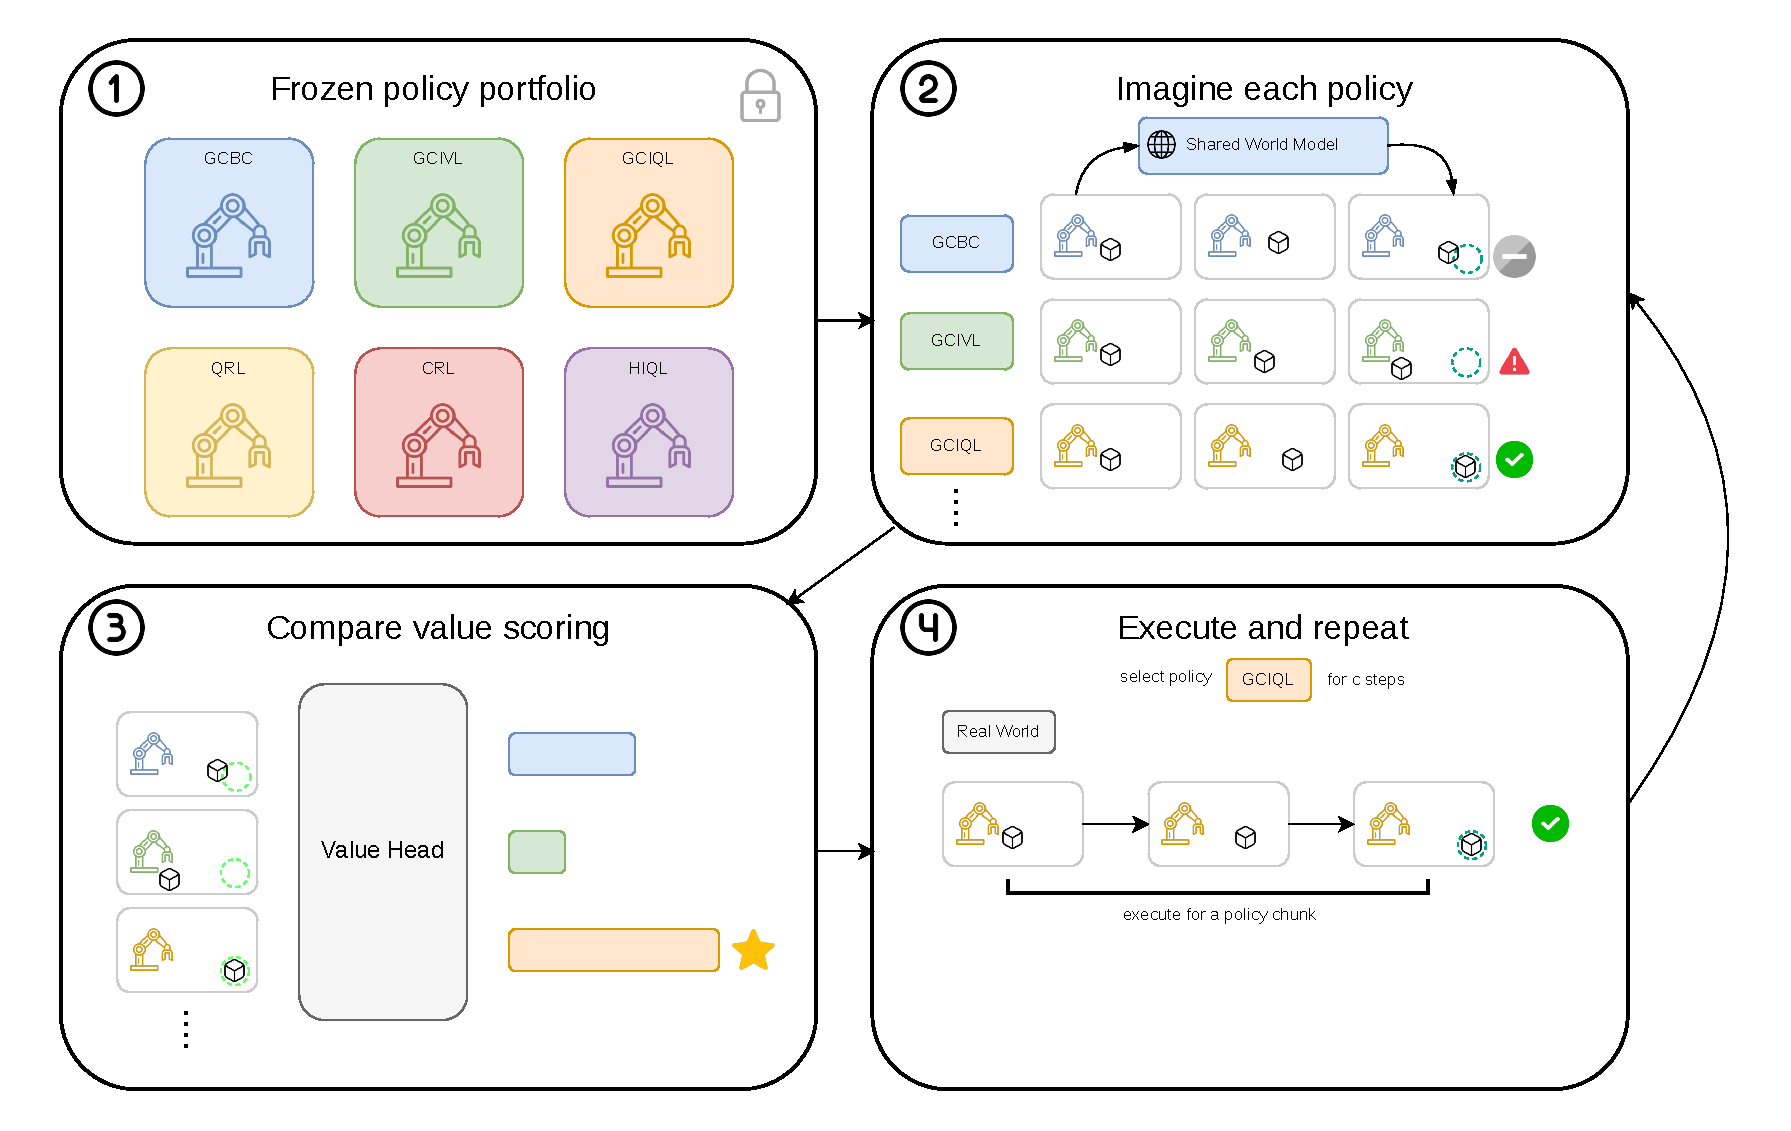
\includegraphics[width=\linewidth]{figures/wmppteaser_optimized.pdf}
    \caption{
    \textbf{WMPP overview.}
    (1) We begin with a frozen portfolio of heterogeneous GCRL policies.
    (2) \wmpp{} imagines the future induced by each policy through a shared
    learned world model.
    (3) A shared goal-conditioned value function scores the predicted futures
    on a common scale.
    (4) The highest-ranked policy is executed for $c$ steps, after which the
    portfolio is re-evaluated and the process repeats.
    }
    \label{fig:overview}
\end{figure}

\section{Related Work}

\paragraph{Goal-conditioned reinforcement learning.}
GCRL learns policies that condition on a desired goal and has been studied with supervised, value-based, contrastive, quasimetric, and hierarchical objectives \citep{eysenbach2022contrastive,wang2023quasimetric,park2023hiql}. Our experiments use the offline setting, where policies are learned from fixed trajectories. OGBench provides common datasets and implementations for several representative learners and shows that their strengths vary across long-horizon navigation, stitching, stochasticity, and manipulation \citep{park2025ogbench}. These works train individual policies; we study how several already-trained policies can be used together at test time.

\paragraph{Test-time planning with frozen goal-conditioned policies.}
Goal-conditioned policies can serve as low-level controllers for planning through intermediate goals \citep{nasiriany2019planning}. Test-Time Graph Search (TTGS) builds a graph over dataset states and supplies a sequence of subgoals to one frozen policy \citep{opryshko2026ttgs}. TTGS and \wmpp{} both improve pretrained GCRL agents at test time, but they address different decisions. TTGS asks \emph{which subgoal should one policy pursue?}; \wmpp{} keeps the final goal fixed and asks \emph{which policy should control the agent now?} The two are complementary.

\paragraph{World models and planning over policies.}
World models are commonly used for action-level planning or to train an amortized policy \citep{schrittwieser2020muzero,hafner2023dreamerv3}. Generalized policy improvement selects among policies when their action-values are comparable \citep{barreto2017successor}. Most closely related, CompPlan learns jumpy successor models and composes a parameterized family of policies, often indexed by subgoals \citep{farebrother2026compplan}. \wmpp{} instead wraps separately trained GCRL algorithms that all receive the same final goal, and uses a shared one-step dynamics model and value function as a common comparison interface across the bank.

\section{Problem Setup}

We consider a controlled Markov process with state space $\calS$, action space $\calA$, goal space $\calG$, transition kernel $p(s'\mid s,a)$, and initial-state distribution $\mu$. A goal-conditioned policy maps a state and goal to an action distribution, $\pi(a\mid s,g)$. The evaluation objective is goal-reaching success.

The agent is given a portfolio (bank) of $M$ frozen policies
\begin{equation}
\PiBank = \{\pi_1,\ldots,\pi_M\}.
\end{equation}
The policies may be trained by different GCRL algorithms, datasets, or random seeds. We assume only black-box action access and a common state, action, and goal interface; their internal values and representations need not be available or comparable.

We also assume a logged trajectory set $\calD$ for training the auxiliary world model and value function. This data may be an offline dataset, a replay buffer, or trajectories collected during policy training. In our experiments, $\calD$ is the OGBench training split and the policies are trained offline, but the policy-portfolio problem itself is not restricted to offline GCRL.

At decision time $t$, an arbiter chooses a policy index $z_t\in\{1,\ldots,M\}$. The selected policy controls the agent for a commitment interval $c$:
\begin{equation}
a_{t+j}\sim \pi_{z_t}(\cdot\mid s_{t+j},g), \qquad j=0,\ldots,c-1.
\end{equation}
The objective is to maximize goal-reaching success while leaving every member of $\PiBank$ unchanged. The central problem is to estimate which policy will produce the most useful future from the current state.

\section{World-Model Policy Portfolios}
\label{sec:method}

\subsection{Learned state-space world model}

For each environment, we train an ensemble of $E$ independently parameterized MLP dynamics models directly in the benchmark state space. Let $\tilde{s}=(s-\mu_s)/\sigma_s$ denote a state normalized by fixed trajectory statistics. Each member predicts a normalized one-step delta,
\begin{align}
\hat{\delta}^{(e)}_t &= f_{\theta_e}(\tilde{s}_t,a_t),\\
\hat{s}^{(e)}_{t+1} &= s_t + \sigma_{\Delta}\hat{\delta}^{(e)}_t+\mu_{\Delta},
\end{align}
where $\mu_{\Delta}$ and $\sigma_{\Delta}$ are fixed statistics of valid logged transitions. Members are trained on $H$-step windows by unrolling their own predictions and penalizing the normalized error at every step,
\begin{equation}
\mathcal{L}_{\mathrm{dyn}} = \frac{1}{E}\sum_{e=1}^{E}
\E_{\tau\sim\calD}
\left[\sum_{h=1}^{H} w_h\left\|\big(\hat{s}^{(e)}_{t+h}-s_{t+h}\big)/\sigma_s\right\|_2^2\right],
\end{equation}
with a curriculum that ramps the effective horizon from $1$ to $H$ over the first $10^5$ updates ($w_h$ uniform over the active steps). The state-space design isolates the arbitration question from visual representation learning and guarantees that predicted states remain valid inputs to all frozen policies.

\subsection{Goal-conditioned metric value function}

The world model predicts candidate futures, but the arbiter still needs a common score. For each ensemble member, the goal-conditioned value is
\begin{equation}
V_{\phi_e}(s,g)
= -\left\|\varphi^{(e)}_{S}(s)-\varphi^{(e)}_{G}(\psi^{(e)}(g))\right\|_2,
\label{eq:metric-value}
\end{equation}
where $\varphi^{(e)}_{S}:\calS\rightarrow\R^d$ and $\varphi^{(e)}_{G}:\R^{d_\psi}\rightarrow\R^d$ are separate state and goal encoders and $\psi^{(e)}$ is a low-dimensional, length-normalized goal representation. Larger values indicate that the state is predicted to be closer to the goal in the learned temporal geometry. The parameterization follows LAVL \citep{kang2026lavl}: separate embeddings compared through a negative Euclidean distance provide a structured inductive bias for imagined out-of-distribution state--goal pairs, while the distinct encoders retain directional reachability, $V(s,g)\neq V(g,s)$ in general.

This parameterization is useful for policy arbitration for two reasons. First, closed-loop model rollouts produce state--goal pairs outside the empirical training support. The latent distance constrains how the scorer extrapolates, reducing the freedom of an unconstrained scalar MLP. This is an inductive bias, not a guarantee of out-of-distribution correctness. Second, goal reachability is directional, which symmetric distances between a single embedding cannot express.

We train the metric value with an expectile temporal-difference objective. For a logged transition $(s,a,s')$ and a relabeled goal $g$, with the sparse reward $r(s,g)=0$ if $s$ attains $g$ and $-1$ otherwise, let
\begin{equation}
\delta_e(s,s',g)
= r(s,g)+\gamma\,m(s,g)\,\bar V_{\bar\phi_e}(s',g)-V_{\phi_e}(s,g),
\end{equation}
where $\bar V$ is a slowly updated target network (Polyak rate $\tau=0.005$) and $m(s,g)=0$ at goal attainment. The loss is
\begin{equation}
\mathcal{L}_{\mathrm{value}}
= \frac{1}{E}\sum_{e=1}^{E}
\E\left[
\left|\kappa-\mathbf{1}\{\delta_e<0\}\right|\delta_e^2
\right],
\label{eq:expectile}
\end{equation}
with expectile $\kappa>0.5$ approximating a maximum over dataset-supported actions. Goals are relabeled from the logged trajectories with the standard OGBench mixture: the current state with probability $0.2$, a geometrically sampled future state of the same trajectory with probability $0.5$, and a uniformly random dataset state with probability $0.3$. The discount and expectile are set per environment family ($\gamma\in\{0.99,0.998,0.999\}$, $\kappa\in\{0.7,0.9\}$; \cref{app:wm}). This training uses no object-specific progress function or simulator predicate.

\subsection{Counterfactual rollout and ranking}

At each arbitration point, every frozen policy is rolled out closed-loop for $k$ model steps, acting deterministically (temperature $0$) on its own imagined states. For policy $i$ and ensemble member $e$,
\begin{align}
\hat{s}^{i,e}_{0} &= s_t,\\
\hat{a}^{i,e}_{h} &= \pi_i(\hat{s}^{i,e}_{h},g),\\
\hat{s}^{i,e}_{h+1} &= \hat{f}_{\theta_e}(\hat{s}^{i,e}_{h},\hat{a}^{i,e}_{h}),
\qquad h=0,\ldots,k-1.
\end{align}
We score the most reachable imagined state along the rollout,
\begin{equation}
S_i(s_t,g)=\max_{1\le h\le k}
\frac{1}{E}\sum_{e=1}^{E}
V_{\phi_e}(\hat{s}^{i,e}_{h},g).
\label{eq:score}
\end{equation}
The max operator lets a policy receive credit for reaching the goal before the end of the planning horizon. The arbiter selects $i^*=\arg\max_i S_i$, executes $\pi_{i^*}$ in the real environment for $c$ steps, and then replans.

\begin{algorithm}[t]
\caption{World-Model Policy Portfolio arbitration}
\label{alg:wmpp}
\begin{algorithmic}[1]
\Require frozen policies $\PiBank$, dynamics ensemble $\{\hat f_{\theta_e}\}_{e=1}^E$, value ensemble $\{V_{\phi_e}\}_{e=1}^E$, goal $g$, planning horizon $k$, commitment $c$
\While{episode not terminated}
    \For{$i=1,\ldots,M$}
        \State Roll out $\pi_i$ for $k$ imagined steps through every ensemble member
        \State Compute $S_i$ with \cref{eq:score}
    \EndFor
    \State $i^*\gets\arg\max_i S_i$
    \State Execute frozen policy $\pi_{i^*}$ in the real environment for up to $c$ steps
\EndWhile
\end{algorithmic}
\end{algorithm}

\paragraph{Budget and the $k{=}c$ diagonal.}
One arbitration costs $M\cdot E\cdot k$ dynamics evaluations and as many value evaluations. Amortized over the commitment interval, the nominal model budget per environment step is $M E k/c$. We always tie the two horizons, $k=c$, so that every configuration costs the same $M E$ model calls per environment step (about $15$--$18$ in our banks). The horizon is therefore a single hyperparameter that trades short-horizon reactivity against long-horizon foresight at zero difference in compute; we sweep $k=c\in\{1,5,10,25,50,100\}$ and report the whole sweep (\cref{app:hyperparams}).

\section{Experimental Setup}
\label{sec:setup}

\paragraph{Benchmark.}
We evaluate on 20 state-based OGBench datasets \citep[v1.2.1;][]{park2025ogbench}: \texttt{antmaze-large-navigate}, \texttt{humanoidmaze-giant-navigate}, \texttt{cube-\{single,\allowbreak double,\allowbreak triple,\allowbreak quadruple\}-\allowbreak\{play,\allowbreak noisy\}}, \texttt{scene-\{play,\allowbreak noisy\}}, and \texttt{puzzle-\{3x3,\allowbreak 4x4,\allowbreak 4x5,\allowbreak 4x6\}-\allowbreak\{play,\allowbreak noisy\}}. The suite spans maze navigation and cube, scene, and puzzle manipulation, and includes both play and noisy data-collection variants. Results for \NumEnvs{} datasets are complete; \texttt{puzzle-4x6-noisy} is pending. OGBench provides a controlled setting in which policies trained with different GCRL objectives share the same observation, action, goal, and evaluation interfaces. We use state observations to isolate policy arbitration from visual representation learning.

\paragraph{Policy bank.}
The portfolio contains the six OGBench reference learners, GCBC, GCIVL, GCIQL, QRL, CRL, and HIQL, each trained with the unmodified reference implementation and the benchmark's per-family hyperparameters for $10^6$ gradient steps. A bank holds one checkpoint per algorithm, and the whole study is replicated over three independent bank seeds. Six datasets (\texttt{cube-triple-\allowbreak\{play,\allowbreak noisy\}}, \texttt{cube-quadruple-play}, \texttt{humanoidmaze-giant-navigate}, \texttt{puzzle-4x4-play}, \texttt{scene-play}) have five-member banks because HIQL is unavailable; we omit rather than impute. All policies remain frozen during auxiliary-model training and evaluation. Individual bank-member scores are listed in \cref{app:bank}.

\paragraph{Auxiliary models.}
The dynamics ensemble ($E=3$) and the metric value ensemble are trained jointly from the corresponding OGBench training split, once per dataset, with fixed normalization statistics stored in the checkpoint. Architecture and training details are in \cref{app:wm}.

\paragraph{Baselines and controls.}
We compare against every individual bank policy and report two quantities: \bestfixed, the algorithm family with the highest mean success over the three seeds (a strong, post-hoc baseline), and \randomswitch, which samples a policy uniformly from the bank at every commitment boundary with the same bank and the same $c$ as \wmpp{} but no learned score and zero model calls. \randomswitch{} tests whether the commitment schedule alone, rather than model-based selection, explains the gains. We do not compare policy-native critics because the bank mixes incompatible objectives and GCBC has no critic.

\paragraph{Protocol and statistics.}
Every number follows the official OGBench evaluation: five evaluation goals per dataset, $50$ episodes per goal, deterministic actions, i.e., $250$ episodes per bank seed and $750$ per method. Every bank policy, \wmpp{}, and \randomswitch{} are evaluated on the same fixed list of episode seeds, so every comparison in the paper is paired per episode. Uncertainty is computed with a hierarchical bootstrap of the per-episode differences that resamples bank seeds and then episodes within seed ($10^4$ resamples, 95\% percentile intervals). We call a difference significant when its interval excludes zero and report raw counts without multiple-comparison correction. The horizon $k{=}c$ is selected per dataset from the sweep by mean success over the three seeds (ties to the smallest $k$); the complete sweep is reported so that sensitivity to this choice is visible (\cref{app:hyperparams}).

\section{Results}

\subsection{Policy portfolios improve goal reaching}

\Cref{tab:main} reports success rates for the strongest single policy, \randomswitch, and \wmpp{}. Averaged over the \NumEnvs{} completed datasets, \wmpp{} reaches \MeanWMPP\% against \MeanBest\% for the best fixed policy and \MeanRandom\% for random switching. \wmpp{} has the highest mean on \NumBetterMean{} of \NumEnvs{} datasets. Against the best policy, the gain is significant on \NumSigUp{} datasets, not significant on \NumNS{}, and significantly negative on \NumSigDown{} (hierarchical bootstrap over seeds and episodes, 95\% intervals; \cref{app:stats}). The largest improvements are on multi-object manipulation: \GainScenePlay{} points on \texttt{scene-play} (\BestScenePlay\% $\rightarrow$ \WmppScenePlay\%), \GainSceneNoisy{} on \texttt{scene-noisy}, \GainCubeDoubleNoisy{} on \texttt{cube-double-noisy}, \GainCubeDoublePlay{} on \texttt{cube-double-play}, and \GainPuzzleFourbyFourNoisy{} on \texttt{puzzle-4x4-noisy}. Smaller but significant gains appear on \texttt{cube-triple-noisy} (\GainCubeTripleNoisy) and \texttt{puzzle-3x3-play} (\GainPuzzleThreebyThreePlay), and \wmpp{} adds \GainCubeSingleNoisy{} points to an already saturated \texttt{cube-single-noisy}. Gains of $2$--$3$ points on \texttt{antmaze-large-navigate} (\GainAntmazeLargeNavigate, on top of a \BestAntmazeLargeNavigate\% baseline), \texttt{puzzle-3x3-noisy}, \texttt{puzzle-4x4-play}, \texttt{puzzle-4x5-play}, and \texttt{puzzle-4x6-play} are consistent in sign but their intervals include zero.

\begin{table}[t]
\caption{\textbf{Success rate (\%) on OGBench under the official protocol} ($5$ goals $\times$ $50$ episodes, $3$ bank seeds; mean $\pm$ std over seeds). \bestfixed{} is the strongest algorithm family in the bank (highest three-seed mean), evaluated on the same episodes as \wmpp{}; \randomswitch{} draws uniformly from the same bank at the same commitment interval as \wmpp{}; \wmpp{} arbitrates over the same frozen bank with the world model. Numbers at or above $95\%$ of the best value in the row are in bold; significance of the \wmpp{} gain over the best policy is assessed with a hierarchical bootstrap over seeds and episodes (\cref{app:stats}). Per-dataset $(k,c)$ are listed in \cref{app:hyperparams}; \texttt{puzzle-4x6-noisy} is pending.}
\label{tab:main}
\centering
\small
\setlength{\tabcolsep}{4.5pt}
\begin{tabular}{llcccc}
\toprule
Family & Dataset & Best Policy & Success Rate & Random Switch & WMPP (Ours) \\
\midrule
\multirow{2}{*}{Maze} & \texttt{antmaze-large-navigate} & HIQL & $\mathbf{90.3 \pm 1.3}$ & $\mathbf{88.3 \pm 2.4}$ & $\mathbf{92.5 \pm 0.2}$ \\
 & \texttt{humanoidmaze-giant-navigate} & CRL & $\mathbf{5.2 \pm 2.9}$ & $2.3 \pm 1.4$ & $4.3 \pm 1.8$ \\
\midrule
\multirow{8}{*}{Cube} & \texttt{cube-single-play} & GCIVL & $\mathbf{49.3 \pm 0.2}$ & $11.9 \pm 3.6$ & $45.6 \pm 2.9$ \\
 & \texttt{cube-single-noisy} & GCIQL & $\mathbf{99.1 \pm 0.5}$ & $\mathbf{95.9 \pm 1.9}$ & $\mathbf{99.9 \pm 0.2}$ \\
 & \texttt{cube-double-play} & GCIQL & $36.1 \pm 5.6$ & $19.7 \pm 1.3$ & $\mathbf{72.8 \pm 1.8}$ \\
 & \texttt{cube-double-noisy} & GCIQL & $25.6 \pm 7.3$ & $26.8 \pm 1.3$ & $\mathbf{60.4 \pm 5.3}$ \\
 & \texttt{cube-triple-play} & CRL & $\mathbf{4.8 \pm 2.7}$ & $3.2 \pm 1.5$ & $3.9 \pm 2.2$ \\
 & \texttt{cube-triple-noisy} & GCIVL & $9.2 \pm 2.4$ & $14.7 \pm 1.8$ & $\mathbf{18.8 \pm 2.1}$ \\
 & \texttt{cube-quadruple-play} & QRL & $0.0 \pm 0.0$ & $0.0 \pm 0.0$ & $0.0 \pm 0.0$ \\
 & \texttt{cube-quadruple-noisy} & CRL & $0.1 \pm 0.2$ & $\mathbf{0.9 \pm 0.7}$ & $0.8 \pm 0.6$ \\
\midrule
\multirow{2}{*}{Scene} & \texttt{scene-play} & GCIQL & $51.9 \pm 2.9$ & $41.5 \pm 2.0$ & $\mathbf{91.2 \pm 0.9}$ \\
 & \texttt{scene-noisy} & GCIVL & $29.6 \pm 1.0$ & $44.8 \pm 3.8$ & $\mathbf{70.7 \pm 4.5}$ \\
\midrule
\multirow{7}{*}{Puzzle} & \texttt{puzzle-3x3-play} & GCIQL & $14.0 \pm 5.3$ & $15.7 \pm 2.4$ & $\mathbf{20.4 \pm 3.1}$ \\
 & \texttt{puzzle-3x3-noisy} & GCIQL & $\mathbf{91.5 \pm 1.4}$ & $73.1 \pm 4.6$ & $\mathbf{93.9 \pm 1.9}$ \\
 & \texttt{puzzle-4x4-play} & GCIQL & $24.1 \pm 3.4$ & $9.3 \pm 2.0$ & $\mathbf{26.7 \pm 4.3}$ \\
 & \texttt{puzzle-4x4-noisy} & GCIQL & $34.0 \pm 3.8$ & $46.0 \pm 4.1$ & $\mathbf{53.6 \pm 3.7}$ \\
 & \texttt{puzzle-4x5-play} & GCIQL & $10.9 \pm 2.4$ & $6.4 \pm 0.9$ & $\mathbf{13.2 \pm 2.0}$ \\
 & \texttt{puzzle-4x5-noisy} & GCIVL & $\mathbf{19.9 \pm 0.2}$ & $11.5 \pm 0.7$ & $\mathbf{20.0 \pm 0.3}$ \\
 & \texttt{puzzle-4x6-play} & GCIVL & $11.3 \pm 0.2$ & $6.3 \pm 1.0$ & $\mathbf{13.6 \pm 1.1}$ \\
\midrule
\multicolumn{3}{l}{Average (19 datasets)} & $31.9$ & $27.3$ & $\mathbf{42.2}$ \\
\bottomrule
\end{tabular}

\end{table}

Two families of null results are expected by construction and we keep them in the table. When every bank member is at the task floor (\texttt{cube-quadruple-\allowbreak\{play,\allowbreak noisy\}}, \texttt{cube-triple-play}, \texttt{humanoidmaze-giant-navigate}), a selector has nothing to select; when a member is saturated (\texttt{cube-single-noisy}, \BestCubeSingleNoisy\%), there is no headroom, and \wmpp{} matches it (\WmppCubeSingleNoisy\%). The only loss of more than one point is \texttt{cube-single-play} (\GainCubeSinglePlay{} points; the interval includes zero), where one policy dominates the bank by a wide margin (GCIVL \BestCubeSinglePlay\%, next best \SecondCubeSinglePlay\%): every switch away from the dominant policy is a cost, and the scorer's occasional ranking errors are not compensated by any complementary behavior. We return to these regimes in \cref{sec:when}.

\subsection{Does the world model matter?}
\label{sec:ablation}

\randomswitch{} shares everything with \wmpp{} except the learned score. Paired per episode, \wmpp{} beats it by \MeanWMPPminusRandom{} points on average and significantly on \NumWMPPvsRandomSig{} of \NumEnvs{} datasets; the contrast is never significantly negative. Random switching by itself is mostly harmful (significantly below the best policy on \NumRandomSigDown{} datasets, \MeanRandom\% mean), which shows that the gains do not come from the commitment schedule or from an implicit ensembling effect of cycling through policies. On a few datasets random switching does help (\texttt{scene-noisy} \GainRandSceneNoisy, \texttt{puzzle-4x4-noisy} \GainRandPuzzleFourbyFourNoisy, \texttt{cube-triple-noisy} \GainRandCubeTripleNoisy): there, every bank member gets stuck in states that another member can leave, and any switching escapes. Model-based selection adds a further \WvsRSceneNoisy, \WvsRPuzzleFourbyFourNoisy, and \WvsRCubeTripleNoisy{} points on top.

We observes interesting results from \randomswitch{}. It is surprisingly good on the small puzzles: if its commitment interval is chosen post hoc, per-step re-drawing ($c=\RandBestCArgPuzzleThreebyThreePlay$) reaches \RandBestCPuzzleThreebyThreePlay\% on \texttt{puzzle-3x3-play}, more than twice the \WmppPuzzleThreebyThreePlay\% of \wmpp{}, and fast cycling also exceeds \wmpp{} a bit on \texttt{puzzle-3x3-noisy} (\RandBestCPuzzleThreebyThreeNoisy\% vs.\ \WmppPuzzleThreebyThreeNoisy\%), \texttt{puzzle-4x5-play} (\RandBestCPuzzleFourbyFivePlay\% vs.\ \WmppPuzzleFourbyFivePlay\%), and \texttt{puzzle-4x6-play} (\RandBestCPuzzleFourbySixPlay\% vs.\ \WmppPuzzleFourbySixPlay\%; \cref{app:random-c}). On these button-pressing tasks the policies fail by stalling rather than by acting wrongly, so rapid re-drawing acts as a restart mechanism that the long-horizon cells selected for \wmpp{} do not exploit. On the mazes, the scene datasets, and the single- and double-cube datasets, \wmpp{} exceeds random switching at every interval; the remaining exceptions are the near-floor triple- and quadruple-cube datasets, where the best random interval is within a few points of \wmpp{}.

\subsection{When does arbitration help?}
\label{sec:when}

\wmpp{} can only select behavior that exists in the bank, so we characterize each bank with quantities that do not require privileged task state. Let $J_i$ denote test success of fixed policy $i$, with $J_{(1)}\ge J_{(2)}\ge\cdots$, and define the best-policy strength $B_{\max}=J_{(1)}$, the dominance gap $D_{\mathrm{gap}}=J_{(1)}-J_{(2)}$, and the number of competent policies $N_{1/2}=\sum_i\mathbf{1}[J_i\ge J_{(1)}/2]$. In addition, by re-evaluating every bank member on the same episodes as \wmpp{} under the official protocol, we compute the \emph{static per-episode oracle} $U$: the success of a hindsight selector that picks, for each episode, the single best policy for that episode and never switches. $U-B_{\max}$ measures how complementary the members' failures are (\cref{app:bank-stats}).

\begin{figure}[t]
    \centering
    \begin{subfigure}[c]{0.44\linewidth}
        \centering
        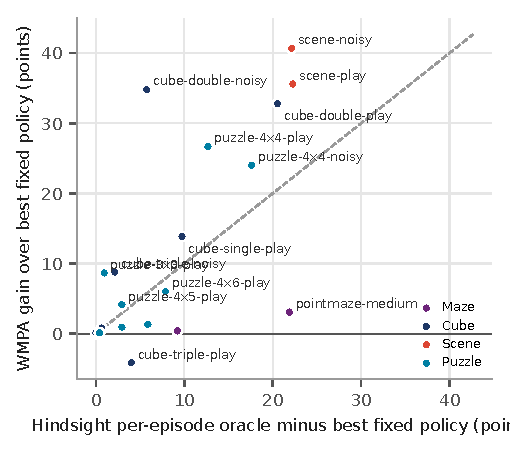
\includegraphics[width=\linewidth]{figures/regimes.pdf}
        \caption{Gain vs.\ complementarity headroom.}
        \label{fig:regimes}
    \end{subfigure}\hfill
    \begin{subfigure}[c]{0.54\linewidth}
        \centering
        \scriptsize
        \setlength{\tabcolsep}{5pt}
        \renewcommand{\arraystretch}{0.92}
        \begin{tabular}{lrrr}
\toprule
Dataset & Best & $U$ & \wmpp \\
\midrule
\texttt{pointmaze-medium-navigate} & $76$ & $98$ & $79$$^{\uparrow}$ \\
\texttt{antmaze-large-navigate} & $90$ & $99$ & $91$$^{\uparrow}$ \\
\midrule
\texttt{cube-single-play} & $71$ & $81$ & $\mathbf{85}$$^{\uparrow}$ \\
\texttt{cube-single-noisy} & $99$ & $100$ & $\mathbf{100}$$^{\uparrow}$ \\
\texttt{cube-double-play} & $36$ & $57$ & $\mathbf{69}$$^{\uparrow}$ \\
\texttt{cube-double-noisy} & $26$ & $31$ & $\mathbf{60}$$^{\uparrow}$ \\
\texttt{cube-triple-play} & $5$ & $9$ & $1$ \\
\texttt{cube-triple-noisy} & $9$ & $11$ & $\mathbf{18}$$^{\uparrow}$ \\
\texttt{cube-quadruple-play} & $0$ & $0$ & $0$ \\
\texttt{cube-quadruple-noisy} & $0$ & $0$ & $\mathbf{0}$$^{\uparrow}$ \\
\midrule
\texttt{scene-play} & $52$ & $74$ & $\mathbf{87}$$^{\uparrow}$ \\
\texttt{scene-noisy} & $30$ & $52$ & $\mathbf{70}$$^{\uparrow}$ \\
\midrule
\texttt{puzzle-3x3-play} & $91$ & $92$ & $\mathbf{100}$$^{\uparrow}$ \\
\texttt{puzzle-3x3-noisy} & $91$ & $97$ & $93$$^{\uparrow}$ \\
\texttt{puzzle-4x4-play} & $24$ & $37$ & $\mathbf{51}$$^{\uparrow}$ \\
\texttt{puzzle-4x4-noisy} & $34$ & $52$ & $\mathbf{58}$$^{\uparrow}$ \\
\texttt{puzzle-4x5-play} & $14$ & $17$ & $\mathbf{18}$$^{\uparrow}$ \\
\texttt{puzzle-4x5-noisy} & $20$ & $20$ & $20$$^{\uparrow}$ \\
\texttt{puzzle-4x6-play} & $11$ & $19$ & $17$$^{\uparrow}$ \\
\texttt{puzzle-4x6-noisy} & $19$ & $22$ & $20$$^{\uparrow}$ \\
\bottomrule
\end{tabular}

        \caption{Static per-episode oracle $U$ (\%), all datasets.}
        \label{tab:oracle}
    \end{subfigure}
    \caption{\textbf{What makes arbitration work?} (a) \wmpp{} gain over the best policy against the headroom $U-B_{\max}$ of a hindsight oracle that picks the best single policy per episode; the dashed line is $y=x$. Points above the line are datasets where within-episode switching composes behavior that no single policy exhibits. (b) Best is \bestfixed{} of \cref{tab:main}, evaluated on the same paired episodes from which $U$ is computed; $^{\uparrow}$ marks the \NumAboveBestPaired{} datasets on which the \wmpp{} point estimate is above the best policy on these episodes, and bold marks the \NumAboveUnionAny{} datasets on which it is above the oracle $U$ itself (point estimates, no significance test; on \NumAboveUnion{} of these the margin over $U$ exceeds one point). A bank with no complementarity (\texttt{puzzle-4x5-noisy}, $U-B_{\max}=\HeadroomPuzzleFourbyFiveNoisy$) yields no gain, and a single dominant policy (\texttt{cube-single-play}) yields a loss. Full statistics in \cref{app:bank-stats}.}
    \label{fig:when}
\end{figure}

Three observations follow (\cref{fig:when}). First, \wmpp{} exceeds the static oracle on \NumAboveUnion{} datasets, by wide margins on \texttt{cube-double-play} (\WmppCubeDoublePlay\% vs.\ $U=\UnionCubeDoublePlay\%$) and \texttt{scene-play} (\WmppScenePlay\% vs.\ \UnionScenePlay\%). No fixed assignment of one policy per episode can reach these numbers: the gains come from composing policies \emph{within} an episode, e.g., one policy that grasps reliably and another that places reliably. Second, the headroom $U-B_{\max}$ is a useful predictor of the null rows. \texttt{puzzle-4x5-noisy} has two near-equal policies (GCIVL and GCIQL, both about $20\%$) but they fail on the same episodes ($U-B_{\max}=\HeadroomPuzzleFourbyFiveNoisy$ points), and arbitration correctly gains nothing (\GainPuzzleFourbyFiveNoisy). Rank statistics alone are misleading here: what matters is whether the members' competencies differ, not whether their scores do. Third, a large dominance gap is the risk case. On \texttt{cube-single-play} ($D_{\mathrm{gap}}=\DgapCubeSinglePlay$ points) the bank offers complementary episodes ($U-B_{\max}=\HeadroomCubeSinglePlay$), but the price of every mis-ranked arbitration is paid against a much stronger incumbent, and the net effect is negative.

\subsection{Sensitivity to the horizon and runtime}

\Cref{app:hyperparams} shows success as a function of $k=c$ for every dataset. The profiles are smooth and unimodal, but their peaks differ by family. Cube, scene, and maze datasets prefer short horizons ($k\le 10$): their dynamics models are trained on $H=5$--$10$ windows, and scoring far beyond the training horizon degrades ranking. Puzzle datasets prefer long horizons ($k\ge 25$), and \texttt{puzzle-3x3-noisy} is the extreme case: the strongest policy's advantage only becomes visible late, and short-horizon scoring is misled by a mid-competence policy that makes faster early progress (\wmpp{} at $k{=}1$: $14.8\%$; at $k{=}100$: \WmppPuzzleThreebyThreeNoisy\%). Because the diagonal has constant compute, this choice is a matter of validity horizon, not budget.

\wmpp{} performs $ME\approx 15$--$18$ dynamics and value evaluations per environment step regardless of $k$. On a single CPU core-set (8 threads, no GPU), this adds $2$--$4$\,ms per environment step over a fixed policy ($\approx0.2$\,ms), i.e., an order of magnitude but still far below the control period of the benchmark tasks. Switch counts, decisions per episode, usage entropy, and latency for every dataset are reported in \cref{app:runtime}.

\section{Discussion}

\paragraph{The world model is a common comparison interface.}
The base policies need not expose comparable critics. \wmpp{} converts each policy into a predicted trajectory in one shared state space, then applies the same metric value to every candidate. The model is used as a judge of closed-loop behavior rather than as an action generator, which sidesteps the compounding-error problem of action-level planning: the actions come from competent closed-loop controllers, and the model only has to rank them.

\paragraph{The value function only needs a useful ordering.}
For arbitration, absolute return calibration is less important than ranking candidate futures correctly. The latent distance gives the scorer a simple geometry, while separate state and goal encoders preserve directional reachability. On \texttt{cube-double-play}, the ranking accuracy of the learned scorer against realized outcomes rises from $0.62$ at $k=5$ to $0.84$ at $k=100$ (\cref{app:diagnostics}), and this is enough to more than double the success rate.

\paragraph{The portfolio sets the ceiling, but switching raises it.}
\wmpp{} does not create a new low-level skill: floors stay floors, and a bank without complementary failures yields no gain. Yet the ceiling is not the best single policy per episode; on \NumAboveUnion{} datasets \wmpp{} exceeds that hindsight oracle, because arbitration composes segments of different policies within one episode.

\section{Limitations}

The current study uses state observations; extending the method to pixels requires a policy-compatible latent world model or a shared visual encoder, and reconstruction quality alone may not imply reliable policy ranking. The auxiliary models are trained separately for each environment, so the present contribution is policy reuse rather than cross-environment transfer. The metric architecture provides an inductive bias for generalization but does not guarantee correct values on out-of-distribution imagined states. The horizon $k{=}c$ is selected per dataset from the test sweep, as OGBench selects per-dataset hyperparameters for the base learners; we report the whole sweep, and the profiles are smooth, but a held-out selection protocol would be stricter. Random switching with a post-hoc interval is competitive on puzzle datasets, where stalling policies benefit from any restart. A single dominant policy can make arbitration a net loss. Finally, simulation results do not establish robustness on real robots, and associations between bank statistics and performance rest on 20 datasets.

\section{Conclusion}

We introduced World-Model Policy Portfolios, a test-time framework that augments frozen goal-conditioned policies with learned policy selection. \wmpp{} rolls each policy forward in a shared world model, ranks the imagined futures with a shared metric value function, and executes the highest-scoring controller for a short commitment interval. It requires no policy retraining and no privileged task-specific progress signal. Under the official OGBench protocol, the portfolio outperforms its strongest fixed member by \MeanGain{} points on average and by $35$--$41$ points on multi-object manipulation, exceeds a hindsight per-episode oracle on \NumAboveUnion{} datasets, and clearly separates from a random-switching control. More broadly, the results motivate a view of world models as evaluators of existing goal-conditioned behaviors, not only as generators of new actions.

\section*{Reproducibility Statement}
Every table and figure is generated by a single script from the evaluation logs; the submission will release configuration files, policy-bank identifiers, world-model checkpoints, fixed episode seed lists, and the scripts that reproduce every number. The appendix specifies architectures, normalization, relabeling distributions, training schedules, per-dataset planning settings, evaluation episodes, statistical procedures, and runtime hardware. An anonymous repository is provided as supplementary material.

\section*{Ethics Statement}
This work studies simulated control benchmarks and does not involve human participants or sensitive personal data. The main foreseeable risk is overgeneralizing simulation findings to safety-critical deployment; the paper therefore limits its claims to post-training arbitration in the evaluated benchmark setting.

\section*{AI Use Statement}
We used AI assistants for editing and for writing analysis and infrastructure code.

\ificlrstyle
  \bibliographystyle{iclr2027_conference}
\else
  \bibliographystyle{plainnat}
\fi
\bibliography{references}

\appendix

\section{Per-Dataset Planning Settings and Horizon Sweep}
\label{app:hyperparams}

\Cref{tab:kc-sweep} lists success for every diagonal cell $k=c\in\{1,5,10,25,50,100\}$ and the selected setting (best mean over three seeds, ties to the smallest $k$). \Cref{fig:kc-profiles} plots the same data together with \randomswitch{} at every interval and the best fixed policy.

\begin{table}[htbp]
\caption{Success rate (\%) of \wmpp{} for every $k=c$ cell; bold marks the selected cell. Every cell uses the same $ME$ model calls per environment step.}
\label{tab:kc-sweep}
\centering
\small
\setlength{\tabcolsep}{4pt}
\begin{tabular}{lccccccc}
\toprule
Dataset & $k{=}c{=}1$ & $k{=}c{=}5$ & $k{=}c{=}10$ & $k{=}c{=}25$ & $k{=}c{=}50$ & $k{=}c{=}100$ & selected \\
\midrule
\texttt{antmaze-large-navigate} & $89.2$ & $\mathbf{92.5}$ & $89.9$ & $82.3$ & $73.5$ & $74.1$ & $(5,5)$ \\
\texttt{humanoidmaze-giant-navigate} & $1.7$ & $2.7$ & $3.7$ & $3.7$ & $\mathbf{4.3}$ & $3.1$ & $(50,50)$ \\
\texttt{cube-single-play} & $\mathbf{45.6}$ & $36.7$ & $31.2$ & $31.2$ & $43.2$ & $42.5$ & $(1,1)$ \\
\texttt{cube-single-noisy} & $99.3$ & $\mathbf{99.9}$ & $99.9$ & $99.2$ & $99.6$ & $99.1$ & $(5,5)$ \\
\texttt{cube-double-play} & $63.5$ & $68.9$ & $\mathbf{72.8}$ & $71.3$ & $65.2$ & $57.3$ & $(10,10)$ \\
\texttt{cube-double-noisy} & $52.9$ & $\mathbf{60.4}$ & $52.0$ & $47.2$ & $40.4$ & $35.5$ & $(5,5)$ \\
\texttt{cube-triple-play} & $0.1$ & $0.7$ & $1.3$ & $1.7$ & $3.6$ & $\mathbf{3.9}$ & $(100,100)$ \\
\texttt{cube-triple-noisy} & $10.7$ & $15.7$ & $17.9$ & $17.7$ & $\mathbf{18.8}$ & $18.3$ & $(50,50)$ \\
\texttt{cube-quadruple-play} & $\mathbf{0.0}$ & $0.0$ & $0.0$ & $0.0$ & $0.0$ & $0.0$ & $(1,1)$ \\
\texttt{cube-quadruple-noisy} & $0.0$ & $0.3$ & $0.0$ & $\mathbf{0.8}$ & $0.5$ & $0.5$ & $(25,25)$ \\
\texttt{scene-play} & $\mathbf{91.2}$ & $87.3$ & $83.6$ & $73.7$ & $64.7$ & $56.8$ & $(1,1)$ \\
\texttt{scene-noisy} & $56.0$ & $\mathbf{70.7}$ & $70.3$ & $64.7$ & $56.4$ & $51.2$ & $(5,5)$ \\
\texttt{puzzle-3x3-play} & $7.3$ & $13.5$ & $14.3$ & $17.7$ & $\mathbf{20.4}$ & $18.7$ & $(50,50)$ \\
\texttt{puzzle-3x3-noisy} & $14.8$ & $24.1$ & $40.5$ & $77.3$ & $91.5$ & $\mathbf{93.9}$ & $(100,100)$ \\
\texttt{puzzle-4x4-play} & $11.2$ & $15.1$ & $16.8$ & $20.5$ & $22.7$ & $\mathbf{26.7}$ & $(100,100)$ \\
\texttt{puzzle-4x4-noisy} & $18.7$ & $34.9$ & $42.8$ & $\mathbf{53.6}$ & $51.5$ & $49.2$ & $(25,25)$ \\
\texttt{puzzle-4x5-play} & $11.9$ & $9.7$ & $9.6$ & $11.7$ & $\mathbf{13.2}$ & $11.5$ & $(50,50)$ \\
\texttt{puzzle-4x5-noisy} & $19.1$ & $19.3$ & $19.6$ & $19.7$ & $\mathbf{20.0}$ & $20.0$ & $(50,50)$ \\
\texttt{puzzle-4x6-play} & $4.8$ & $11.2$ & $13.1$ & $11.5$ & $13.2$ & $\mathbf{13.6}$ & $(100,100)$ \\
\bottomrule
\end{tabular}

\end{table}

\begin{figure}[htbp]
    \centering
    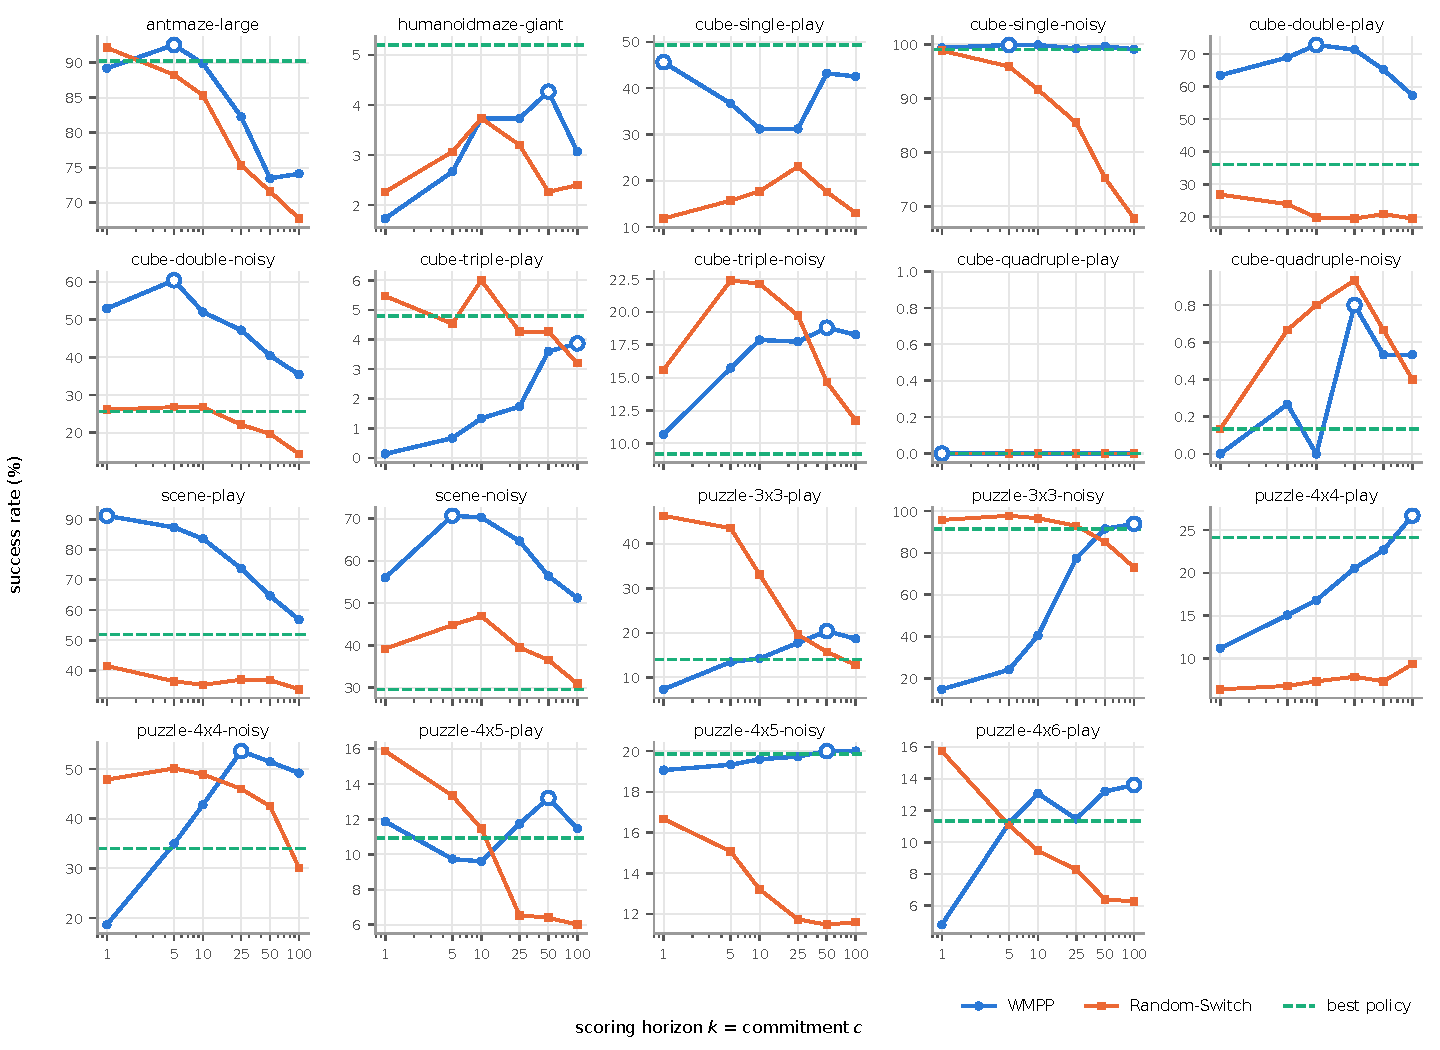
\includegraphics[width=\linewidth]{figures/kc_profiles.pdf}
    \caption{\textbf{Success as a function of the horizon $k=c$} for \wmpp{} (blue; open marker = selected cell) and \randomswitch{} (orange), with the best fixed policy as a dashed line. Cube, scene, and maze datasets peak at short horizons; puzzle datasets peak at long horizons.}
    \label{fig:kc-profiles}
\end{figure}

\section{Random Switching at Every Commitment Interval}
\label{app:random-c}

\Cref{tab:random-c} reports \randomswitch{} for every interval. The main text pairs it with \wmpp{} at the selected $c$ (underlined). The last column shows the best random-switching result over $c$ minus the \wmpp{} result; it is positive on \NumRandomBestCBeats{} datasets, mostly puzzles, where fast cycling acts as a restart heuristic.

\begin{table}[htbp]
\caption{\randomswitch{} success rate (\%) at every commitment interval $c$. Every interval is evaluated on every dataset ($250$ episodes $\times$ $3$ bank seeds, the same episodes as \wmpp{}). Numbers at or above $95\%$ of the best value in the row (\randomswitch{} at any $c$ or \wmpp{}) are in bold; the underlined entry is the interval paired with \wmpp{} in \cref{tab:main} (the selected $c$).}
\label{tab:random-c}
\centering
\small
\setlength{\tabcolsep}{4pt}
\begin{tabular}{lcccccccc}
\toprule
Dataset & $c{=}1$ & $c{=}5$ & $c{=}10$ & $c{=}25$ & $c{=}50$ & $c{=}100$ & \wmpp & best Random $-$ \wmpp \\
\midrule
\texttt{antmaze-large-navigate} & $\mathbf{92.1}$ & \underline{$\mathbf{88.3}$} & $85.3$ & $75.3$ & $71.6$ & $67.7$ & $\mathbf{92.5}$ & $-0.4$ \\
\texttt{humanoidmaze-giant-navigate} & $2.3$ & $3.1$ & $3.7$ & $3.2$ & \underline{$2.3$} & $2.4$ & $\mathbf{4.3}$ & $-0.5$ \\
\texttt{cube-single-play} & \underline{$11.9$} & $15.7$ & $17.7$ & $23.1$ & $17.6$ & $13.1$ & $\mathbf{45.6}$ & $-22.5$ \\
\texttt{cube-single-noisy} & $\mathbf{98.8}$ & \underline{$\mathbf{95.9}$} & $91.6$ & $85.5$ & $75.2$ & $67.7$ & $\mathbf{99.9}$ & $-1.1$ \\
\texttt{cube-double-play} & $26.8$ & $23.9$ & \underline{$19.7$} & $19.5$ & $20.8$ & $19.5$ & $\mathbf{72.8}$ & $-46.0$ \\
\texttt{cube-double-noisy} & $26.1$ & \underline{$26.8$} & $26.8$ & $22.1$ & $19.7$ & $14.4$ & $\mathbf{60.4}$ & $-33.6$ \\
\texttt{cube-triple-play} & $5.5$ & $4.5$ & $\mathbf{6.0}$ & $4.3$ & $4.3$ & \underline{$3.2$} & $3.9$ & $2.1$ \\
\texttt{cube-triple-noisy} & $15.6$ & $\mathbf{22.4}$ & $\mathbf{22.1}$ & $19.7$ & \underline{$14.7$} & $11.7$ & $18.8$ & $3.6$ \\
\texttt{cube-quadruple-play} & \underline{$0.0$} & $0.0$ & $0.0$ & $0.0$ & $0.0$ & $0.0$ & $0.0$ & $0.0$ \\
\texttt{cube-quadruple-noisy} & $0.1$ & $0.7$ & $0.8$ & \underline{$\mathbf{0.9}$} & $0.7$ & $0.4$ & $0.8$ & $0.1$ \\
\texttt{scene-play} & \underline{$41.5$} & $36.4$ & $35.2$ & $36.9$ & $36.8$ & $33.7$ & $\mathbf{91.2}$ & $-49.7$ \\
\texttt{scene-noisy} & $39.2$ & \underline{$44.8$} & $46.9$ & $39.5$ & $36.5$ & $30.9$ & $\mathbf{70.7}$ & $-23.7$ \\
\texttt{puzzle-3x3-play} & $\mathbf{46.3}$ & $43.5$ & $33.1$ & $19.6$ & \underline{$15.7$} & $12.8$ & $20.4$ & $25.9$ \\
\texttt{puzzle-3x3-noisy} & $\mathbf{95.7}$ & $\mathbf{97.7}$ & $\mathbf{96.5}$ & $\mathbf{92.9}$ & $85.2$ & \underline{$73.1$} & $\mathbf{93.9}$ & $3.9$ \\
\texttt{puzzle-4x4-play} & $6.4$ & $6.8$ & $7.3$ & $7.9$ & $7.3$ & \underline{$9.3$} & $\mathbf{26.7}$ & $-17.3$ \\
\texttt{puzzle-4x4-noisy} & $47.9$ & $50.1$ & $48.9$ & \underline{$46.0$} & $42.5$ & $30.1$ & $\mathbf{53.6}$ & $-3.5$ \\
\texttt{puzzle-4x5-play} & $\mathbf{15.9}$ & $13.3$ & $11.5$ & $6.5$ & \underline{$6.4$} & $6.0$ & $13.2$ & $2.7$ \\
\texttt{puzzle-4x5-noisy} & $16.7$ & $15.1$ & $13.2$ & $11.7$ & \underline{$11.5$} & $11.6$ & $\mathbf{20.0}$ & $-3.3$ \\
\texttt{puzzle-4x6-play} & $\mathbf{15.7}$ & $11.1$ & $9.5$ & $8.3$ & $6.4$ & \underline{$6.3$} & $13.6$ & $2.1$ \\
\bottomrule
\end{tabular}

\end{table}

\section{Frozen Policy Bank Performance}
\label{app:bank}

\Cref{tab:bank} lists the success of every bank member under the official protocol on the shared episode seeds (mean over the three bank seeds) next to \wmpp{}. Each checkpoint's own OGBench evaluation at the end of training, an independent draw of $250$ episodes per seed, differs from these numbers by at most \MaxAbsBaselineDiff{} points (mean absolute difference \MeanAbsBaselineDiff) and selects the same best family on \NumBestFamilySame{} of \NumEnvs{} datasets. These numbers document the heterogeneity that motivates a portfolio: the best algorithm differs across datasets (HIQL on the maze, GCIVL or GCIQL on manipulation, CRL where everything is near the floor), and within a dataset the second-best member is often close.

\begin{table}[htbp]
\caption{Success rate (\%) of each fixed policy (algorithm family, mean over three seeds, official protocol on the shared episode seeds) and of \wmpp{}. Numbers at or above $95\%$ of the best value in the row are in bold; a dash denotes an unavailable checkpoint.}
\label{tab:bank}
\centering
\small
\setlength{\tabcolsep}{4pt}
\begin{tabular}{lccccccc}
\toprule
Dataset & GCBC & GCIVL & GCIQL & QRL & CRL & HIQL & \wmpp \\
\midrule
\texttt{antmaze-large-navigate} & $23.2$ & $19.5$ & $36.7$ & $78.1$ & $86.3$ & $\mathbf{90.3}$ & $\mathbf{92.5}$ \\
\texttt{humanoidmaze-giant-navigate} & $0.5$ & $0.0$ & $0.5$ & $0.8$ & $\mathbf{5.2}$ & -- & $4.3$ \\
\texttt{cube-single-play} & $6.4$ & $\mathbf{49.3}$ & $2.3$ & $0.3$ & $0.4$ & $12.1$ & $45.6$ \\
\texttt{cube-single-noisy} & $8.1$ & $70.8$ & $\mathbf{99.1}$ & $33.2$ & $39.7$ & $40.4$ & $\mathbf{99.9}$ \\
\texttt{cube-double-play} & $2.0$ & $34.7$ & $36.1$ & $1.5$ & $9.1$ & $5.1$ & $\mathbf{72.8}$ \\
\texttt{cube-double-noisy} & $0.7$ & $14.3$ & $25.6$ & $3.1$ & $2.7$ & $2.1$ & $\mathbf{60.4}$ \\
\texttt{cube-triple-play} & $1.3$ & $1.3$ & $2.1$ & $0.0$ & $\mathbf{4.8}$ & -- & $3.9$ \\
\texttt{cube-triple-noisy} & $2.1$ & $9.2$ & $2.1$ & $1.7$ & $0.9$ & -- & $\mathbf{18.8}$ \\
\texttt{cube-quadruple-play} & $0.0$ & $0.0$ & $0.0$ & $0.0$ & $0.0$ & -- & $0.0$ \\
\texttt{cube-quadruple-noisy} & $0.0$ & $0.0$ & $0.0$ & $0.0$ & $0.1$ & $0.0$ & $\mathbf{0.8}$ \\
\texttt{scene-play} & $3.7$ & $42.3$ & $51.9$ & $6.1$ & $22.0$ & -- & $\mathbf{91.2}$ \\
\texttt{scene-noisy} & $1.9$ & $29.6$ & $26.8$ & $6.1$ & $0.4$ & $26.1$ & $\mathbf{70.7}$ \\
\texttt{puzzle-3x3-play} & $2.3$ & $3.1$ & $14.0$ & $0.1$ & $12.5$ & $12.0$ & $\mathbf{20.4}$ \\
\texttt{puzzle-3x3-noisy} & $1.1$ & $37.9$ & $\mathbf{91.5}$ & $0.1$ & $30.9$ & $57.3$ & $\mathbf{93.9}$ \\
\texttt{puzzle-4x4-play} & $0.0$ & $11.6$ & $24.1$ & $0.0$ & $0.7$ & -- & $\mathbf{26.7}$ \\
\texttt{puzzle-4x4-noisy} & $0.0$ & $19.2$ & $34.0$ & $0.0$ & $0.0$ & $12.3$ & $\mathbf{53.6}$ \\
\texttt{puzzle-4x5-play} & $0.3$ & $5.6$ & $10.9$ & $0.0$ & $7.6$ & $4.0$ & $\mathbf{13.2}$ \\
\texttt{puzzle-4x5-noisy} & $0.0$ & $\mathbf{19.9}$ & $\mathbf{19.7}$ & $0.0$ & $5.3$ & $3.3$ & $\mathbf{20.0}$ \\
\texttt{puzzle-4x6-play} & $0.1$ & $11.3$ & $1.3$ & $0.0$ & $2.9$ & $3.2$ & $\mathbf{13.6}$ \\
\bottomrule
\end{tabular}

\end{table}

\section{World-Model Architecture and Training Details}
\label{app:wm}

\paragraph{Data.} Each auxiliary model is trained on the OGBench training split of its dataset, with the benchmark's validation split used only for monitoring. Observation and one-step-delta statistics ($\mu_s,\sigma_s,\mu_\Delta,\sigma_\Delta$) are computed once from valid training transitions and stored in the checkpoint.

\paragraph{Dynamics ensemble.} $E=3$ members with disjoint parameters; each is an MLP with three hidden layers of width $512$, GELU activations, and layer normalization, mapping the normalized state and action to a normalized delta of the full observation vector (observation dimension $28$--$115$ depending on the dataset). Training unrolls each member for $H$ steps ($H=5$ for cube, scene, and puzzle; $H=10$ for the two mazes) with a curriculum that increases the unrolled horizon from $1$ to $H$ over the first $10^5$ steps.

\paragraph{Metric value head.} Per member, a goal representation $\psi$ (MLP $512\times3\rightarrow10$, length-normalized to $\sqrt{10}$), a state encoder $\varphi_S$ and a goal encoder $\varphi_G$ (each MLP $512\times3\rightarrow64$), with $V=-\|\varphi_S(s)-\varphi_G(\psi(g))\|_2$ following LAVL \citep{kang2026lavl}. Target networks are Polyak-averaged with $\tau=0.005$. Goal relabeling uses the OGBench value-goal mixture ($0.2$ current / $0.5$ geometric future / $0.3$ random). Rewards are $0$ at goal attainment and $-1$ otherwise; the bootstrap mask is zero at attainment. Per family: $\gamma=0.99$, $\kappa=0.7$ for cube and puzzle; $\gamma=0.998$, $\kappa=0.7$ with LAVL's local-smoothness regularizer (weight $10$) for scene; $\gamma=0.999$, $\kappa=0.9$ for the mazes (smoothness weight $10$ on \texttt{antmaze-large}, $0$ on \texttt{humanoidmaze-giant}).

\paragraph{Optimization.} Dynamics and value losses are summed with unit weights and optimized with Adam (learning rate $3\times10^{-4}$), batch size $1024$, for $10^6$ steps on a single H100 MIG slice (about $4$--$8$ hours per dataset). The $10^6$-step checkpoint is used everywhere except \texttt{antmaze-large}, which uses the $9\times10^5$-step checkpoint. One world model per dataset is shared by all three bank seeds. The same code path serves both training and test-time imagination, so predicted states are directly consumable by every frozen policy.

\section{Bank Statistics and the Static Per-Episode Oracle}
\label{app:bank-stats}

\Cref{tab:bank-stats} lists, per dataset, the bank statistics of \cref{sec:when}. $B_{\max}$, $D_{\mathrm{gap}}$, and $N_{1/2}$ are computed from the scores of \cref{tab:bank}. Because every bank member is evaluated on the same \OracleEpisodes{} episodes per dataset ($5$ goals $\times$ \OracleEpsPerGoal{} episodes $\times$ $3$ bank seeds) as \wmpp{} and \randomswitch{}, the static per-episode oracle needs no additional runs: $U$ is the mean over these episodes of $\max_i \mathbf{1}[\text{policy } i \text{ succeeds}]$, and $U-B_{\max}$ is the headroom available to any per-episode selector that does not switch within an episode. When we say that \wmpp{} exceeds the oracle, we count datasets where it does so by at least one point (\NumAboveUnion{} datasets); it is numerically above $U$ on \NumAboveUnionAny{}, the remainder being floor or saturated datasets where the difference is below one point.

\begin{table}[htbp]
\caption{Bank statistics and the static per-episode oracle (\%). $U$ is the success of a hindsight selector that picks the best single policy for each episode; $U-B_{\max}$ is the headroom available to any per-episode selector without within-episode switching. \wmpp{} and $\Delta$\wmpp{} are the numbers of \cref{tab:main}.}
\label{tab:bank-stats}
\centering
\small
\setlength{\tabcolsep}{4pt}
\begin{tabular}{lccccc r}
\toprule
Dataset & $B_{\max}$ & $D_{\mathrm{gap}}$ & $U$ (oracle) & $U-B_{\max}$ & \wmpp & $\Delta$\wmpp{} [95\% CI] \\
\midrule
\texttt{pointmaze-medium-navigate} & $76 \pm 17$ & $2$ & $\mathbf{98 \pm 1}$ & $22$ & $79 \pm 3$ & +3 [-17, +17] \\
\texttt{antmaze-large-navigate} & $90 \pm 3$ & $4$ & $\mathbf{99 \pm 1}$ & $9$ & $91 \pm 3$ & +0 [-3, +4] \\
\texttt{cube-single-play} & $71 \pm 3$ & $22$ & $\mathbf{81 \pm 3}$ & $10$ & $\mathbf{85 \pm 3}$ & +14 [+10, +18]* \\
\texttt{cube-single-noisy} & $\mathbf{99 \pm 1}$ & $28$ & $\mathbf{100 \pm 0}$ & $1$ & $\mathbf{100 \pm 0}$ & +1 [+0, +2]* \\
\texttt{cube-double-play} & $36 \pm 7$ & $1$ & $57 \pm 6$ & $21$ & $\mathbf{69 \pm 3}$ & +33 [+25, +40]* \\
\texttt{cube-double-noisy} & $26 \pm 9$ & $11$ & $31 \pm 6$ & $6$ & $\mathbf{60 \pm 7}$ & +35 [+30, +40]* \\
\texttt{cube-triple-play} & $5 \pm 3$ & $2$ & $\mathbf{9 \pm 3}$ & $4$ & $1 \pm 1$ & -4 [-8, -1]* \\
\texttt{cube-triple-noisy} & $9 \pm 3$ & $7$ & $11 \pm 3$ & $2$ & $\mathbf{18 \pm 3}$ & +9 [+6, +12]* \\
\texttt{cube-quadruple-play} & $0 \pm 0$ & $0$ & $0 \pm 0$ & $0$ & $0 \pm 0$ & +0 [+0, +0] \\
\texttt{cube-quadruple-noisy} & $0 \pm 0$ & $0$ & $0 \pm 0$ & $0$ & $\mathbf{0 \pm 0}$ & +0 [-1, +1] \\
\texttt{scene-play} & $52 \pm 5$ & $9$ & $74 \pm 6$ & $22$ & $\mathbf{87 \pm 4}$ & +36 [+30, +41]* \\
\texttt{scene-noisy} & $30 \pm 3$ & $3$ & $52 \pm 4$ & $22$ & $\mathbf{70 \pm 5}$ & +41 [+36, +45]* \\
\texttt{puzzle-3x3-play} & $91 \pm 4$ & $79$ & $92 \pm 3$ & $1$ & $\mathbf{100 \pm 0}$ & +9 [+5, +13]* \\
\texttt{puzzle-3x3-noisy} & $91 \pm 3$ & $34$ & $\mathbf{97 \pm 2}$ & $6$ & $\mathbf{93 \pm 2}$ & +1 [-1, +4] \\
\texttt{puzzle-4x4-play} & $24 \pm 5$ & $13$ & $37 \pm 5$ & $13$ & $\mathbf{51 \pm 8}$ & +27 [+18, +36]* \\
\texttt{puzzle-4x4-noisy} & $34 \pm 5$ & $15$ & $52 \pm 7$ & $18$ & $\mathbf{58 \pm 11}$ & +24 [+16, +32]* \\
\texttt{puzzle-4x5-play} & $14 \pm 3$ & $9$ & $17 \pm 3$ & $3$ & $\mathbf{18 \pm 3}$ & +4 [+3, +6]* \\
\texttt{puzzle-4x5-noisy} & $\mathbf{20 \pm 3}$ & $0$ & $\mathbf{20 \pm 3}$ & $0$ & $\mathbf{20 \pm 3}$ & +0 [+0, +1] \\
\texttt{puzzle-4x6-play} & $11 \pm 2$ & $0$ & $\mathbf{19 \pm 3}$ & $8$ & $17 \pm 3$ & +6 [+3, +9]* \\
\texttt{puzzle-4x6-noisy} & $19 \pm 3$ & $1$ & $\mathbf{22 \pm 3}$ & $3$ & $20 \pm 3$ & +1 [-0, +2] \\
\bottomrule
\end{tabular}

\end{table}

\section{Selection Behavior and Runtime}
\label{app:runtime}

\Cref{tab:runtime} reports how the portfolio is used: episode length, switches per episode for \wmpp{} and \randomswitch, arbitration decisions per episode, world-model calls per environment step (dynamics; value calls are identical), the entropy of the policy-usage distribution (bits; $\log_2 6\approx2.58$ for uniform usage of a six-member bank), and wall-clock latency per environment step. Latency was measured on the evaluation nodes (AMD EPYC 9135, 8 threads, JAX on CPU, no GPU) and includes batched policy inference, dynamics and value evaluation, and the winner's action. \wmpp{} switches less often than \randomswitch{} at the same interval (it frequently re-selects the incumbent), and its usage entropy is high on the datasets with the largest gains, i.e., the gains come from genuinely mixing policies rather than from re-discovering the best fixed one.

\begin{table}[htbp]
\caption{Selection behavior and runtime of \wmpp{} (selected $(k,c)$) and \randomswitch{} (same $c$).}
\label{tab:runtime}
\centering
\scriptsize
\setlength{\tabcolsep}{3pt}
\begin{tabular}{lcccccccccc}
\toprule
 & & & \multicolumn{2}{c}{switches/ep} & & & & \multicolumn{3}{c}{ms/step (CPU)} \\
\cmidrule(lr){4-5}\cmidrule(lr){9-11}
Dataset & $(k,c)$ & ep.\ len & \wmpp & Rand. & decisions/ep & WM calls/step & usage $H$ (bits) & \wmpp & Rand. & fixed \\
\midrule
\texttt{antmaze-large-navigate} & $(5,5)$ & 464 & 67.7 & 93.9 & 93.1 & 18.1 & 2.54 & 2.60 & 0.17 & 0.15 \\
\texttt{humanoidmaze-giant-navigate} & $(50,50)$ & 3965 & 50.0 & 62.9 & 79.3 & 15.0 & 2.18 & 2.10 & 0.20 & 0.15 \\
\texttt{cube-single-play} & $(1,1)$ & 132 & 67.4 & 154.8 & 132.0 & 18.0 & 2.52 & 3.68 & 0.27 & 0.22 \\
\texttt{cube-single-noisy} & $(5,5)$ & 46 & 3.7 & 13.0 & 9.5 & 18.8 & 1.61 & 3.24 & 0.24 & 0.30 \\
\texttt{cube-double-play} & $(10,10)$ & 257 & 18.8 & 37.0 & 26.0 & 18.2 & 2.53 & 2.87 & 0.23 & 0.22 \\
\texttt{cube-double-noisy} & $(5,5)$ & 310 & 41.4 & 69.9 & 62.3 & 18.1 & 2.45 & 2.89 & 0.23 & 0.34 \\
\texttt{cube-triple-play} & $(100,100)$ & 975 & 5.9 & 7.1 & 9.8 & 15.0 & 2.24 & 2.08 & 0.22 & 0.20 \\
\texttt{cube-triple-noisy} & $(50,50)$ & 866 & 9.3 & 13.7 & 17.4 & 15.1 & 2.15 & 1.93 & 0.21 & 0.25 \\
\texttt{cube-quadruple-play} & $(1,1)$ & 1000 & 405.4 & 799.9 & 1000.0 & 15.0 & 2.14 & 3.03 & 0.27 & 0.21 \\
\texttt{cube-quadruple-noisy} & $(25,25)$ & 999 & 24.4 & 32.6 & 39.9 & 18.0 & 2.55 & 2.18 & 0.22 & 0.35 \\
\texttt{scene-play} & $(1,1)$ & 247 & 134.6 & 475.5 & 247.5 & 15.0 & 2.31 & 3.95 & 0.57 & 0.20 \\
\texttt{scene-noisy} & $(5,5)$ & 363 & 41.5 & 89.3 & 72.9 & 18.1 & 2.48 & 2.59 & 0.25 & 0.19 \\
\texttt{puzzle-3x3-play} & $(50,50)$ & 430 & 6.0 & 6.7 & 8.7 & 18.2 & 2.51 & 2.06 & 0.20 & 0.23 \\
\texttt{puzzle-3x3-noisy} & $(100,100)$ & 123 & 0.6 & 1.9 & 1.7 & 24.7 & 2.11 & 4.38 & 0.27 & 0.27 \\
\texttt{puzzle-4x4-play} & $(100,100)$ & 442 & 2.2 & 3.1 & 4.5 & 15.4 & 1.87 & 2.16 & 0.39 & 0.23 \\
\texttt{puzzle-4x4-noisy} & $(25,25)$ & 315 & 8.5 & 12.7 & 12.8 & 18.4 & 2.30 & 3.17 & 0.30 & 0.20 \\
\texttt{puzzle-4x5-play} & $(50,50)$ & 897 & 11.6 & 15.0 & 18.0 & 18.1 & 2.49 & 2.16 & 0.24 & 0.20 \\
\texttt{puzzle-4x5-noisy} & $(50,50)$ & 813 & 9.7 & 14.4 & 16.4 & 18.1 & 2.48 & 2.61 & 0.22 & 0.21 \\
\texttt{puzzle-4x6-play} & $(100,100)$ & 909 & 5.9 & 7.1 & 9.2 & 18.1 & 2.47 & 2.32 & 0.26 & 0.20 \\
\bottomrule
\end{tabular}

\end{table}

\section{Statistical Procedure}
\label{app:stats}

For each dataset and method we have three bank seeds with $250$ episodes each ($5$ evaluation goals $\times$ $50$ episodes, deterministic episode seeds shared across methods). Success is a binary outcome per episode.

\paragraph{Contrasts.} Every bank policy, \wmpp{}, and \randomswitch{} are run on the same episode seeds, so every contrast (method vs.\ best policy and method vs.\ method) is computed on per-episode success differences: we resample bank seeds with replacement, then episodes within each selected seed, and recompute the mean difference; $10^4$ resamples give a 95\% percentile interval. Point estimates are the plain means. We re-evaluate the bank policies rather than quoting each checkpoint's own end-of-training OGBench evaluation (an independent draw of $250$ episodes per seed) so that the comparison is paired; the two agree to within \MaxAbsBaselineDiff{} points across all bank members and datasets (\cref{app:bank}).

\paragraph{Significance.} A contrast is called significant when the interval excludes zero. We report counts over datasets without multiple-comparison correction; with $19$ datasets, one or two spurious significant rows are expected under the null, which does not affect the qualitative conclusions (\NumSigUp{} significant gains, several exceeding $30$ points).

\paragraph{Software.} JAX/Flax with the unmodified OGBench v1.2.1 implementations for all policies; MuJoCo 3.1.6.

\section{Prediction and Ranking Diagnostics}
\label{app:diagnostics}

To check that the learned scorer ranks policies for the right reason, we collected a dynamic oracle on \texttt{cube-double-play}: from $172$ decision states along executed episodes, every bank policy was rolled out in the real simulator, and the realized outcome of each policy was recorded. The \wmpp{} score (\cref{eq:score}) computed from the world model at the same states was then compared with the realized ordering. Pairwise ranking accuracy over discordant policy pairs rises with the scoring horizon, from $0.62$ at $k=5$ and $0.64$ at $k=10$ to $0.71$ at $k=20$, $0.79$ at $k=50$, and $0.84$ at $k=100$ ($95\%$ intervals of about $\pm0.04$), and the ensemble disagreement of the dynamics model correlates with its open-loop error (Spearman $0.86$). These diagnostics use no privileged information at test time; they were used only to validate the scorer and are reported for the dataset where the oracle was collected.

\section{Failure Analysis}
\label{app:failures}

The complete matrix contains three boundary regimes, all visible in \cref{tab:main,tab:bank-stats}. \emph{Saturation:} when a fixed policy already solves the task (\texttt{cube-single-noisy}, \BestCubeSingleNoisy\%), arbitration has no headroom and \wmpp{} matches it (\WmppCubeSingleNoisy\%). \emph{Floor:} when every policy is near zero (\texttt{cube-quadruple-\allowbreak\{play,\allowbreak noisy\}}, \texttt{cube-triple-play}, \texttt{humanoidmaze-giant-navigate}), a selector cannot create behavior absent from the bank, and every method stays at the floor. \emph{Dominance:} when one policy is much stronger than the rest (\texttt{cube-single-play}, GCIVL \BestCubeSinglePlay\% against \SecondCubeSinglePlay\% for the runner-up), the best cell is $k=c=1$, which keeps the arbiter as reactive as possible, but the result is still a loss of \GainCubeSinglePlay{} points (the only dataset where the point estimate is below the best policy by more than one point, although the interval includes zero); random switching loses \GainRandCubeSinglePlay{} on the same dataset. A practical safeguard would be to include the incumbent's own imagined score as a hysteresis threshold; we leave this to future work. \emph{No complementarity:} \texttt{puzzle-4x5-noisy} has two equally strong policies that fail on the same episodes, and arbitration neither helps nor hurts.

\TODO{Add qualitative timelines (policy chain, score traces, outcome) for three successful arbitration cases and three failures, using the recorded policy chains; include \texttt{cube-single-play}, one floor case, and one model-prediction failure.}

\end{document}
